\section{Circular density deconvolution}\label{INTRO_CIRCULARDECONVOLUTION}\label{bm:ak}

Let $X$ and $\epsilon$ be circular random variables (that is to say, taking values in the unit circle), and we describe their position by a measure of angle taking values in $[0,1[$; we denote $\mathds{P}_{X}$ and $\mathds{P}_{\epsilon}$ the respective distributions of these measures of angle.
Assume that $\P_{X}$ and $\P_{\epsilon}$ admit respective densities $f$ and $h$ with respect to the Lebesgue measure on $[0, 1]$, denoted $\mu$ and we denote $\mathcal{B}$ the Borel $\sigma$-algebra on $[0, 1]$.

\begin{de}{\textsc{Modular addition}\\}\label{DE_INTRO_CIRCULARDECONVOLUTION_MODADD}
From now on we denote by $\Box$ the modular addition on $[0,1[$. That is to say, for any $x$ and $y$ in $[0, 1[$, $x\Box y = x + y - \lfloor x + y \rfloor$.
\assEnd
\end{de}

We want to estimate $f$ while observing replications of the random variable $Y = X \Box \epsilon$ which distribution we denote $\P_{Y}$.
One would notice that $\mathds{P}_{Y}$ is given, for any $A$ in $\mathcal{B}$, by $\mathds{P}_{Y}(A) = (\mathds{P}_{X} \star \mathds{P}_{\epsilon})(A) = \int_{[0,1[}\int_{[0,1[} \mathds{1}_{A}(x \Box s)\d\mathds{P}_{X}(x)\d\mathds{P}_{\epsilon}(s)$.
Moreover, $\P_{Y}$ also admits a density with respect to the Lebesgue measure, denoted $g$ and for any $y$ in $[0, 1]$, it is given by $g(y) = (f \star h)(y) = \int\nolimits_{0}^{1} f(y \Box (- s)) h(s)\d\mu(s)$.
Indeed, for any $\mu$-measurable and $\mu$-almost surely bounded function $t$, we have
\begin{alignat*}{3}
&\mathds{E}\left[t(Y)\right] &&=&& \mathds{E}\left[t(X \Box \epsilon)\right] = \int_{0}^{1}\int_{0}^{1} t(x \Box s) \d\mathds{P}_{X}(x)\d\mathds{P}_{\epsilon}(s)\\
& &&=&&\int_{0}^{1}\int_{0}^{1} t(y) \d\mathds{P}_{X}(y \Box (-s))\d\mathds{P}_{\epsilon}(s) = \int_{0}^{1} t(y) \int_{0}^{1} \d\mathds{P}_{\epsilon}(s) \d\mathds{P}_{X}(y \Box (-s))\\
& &&=&&\int_{0}^{1} t(y) \int_{0}^{1}f(y \Box (- s)) h(s)\d\mu(s) \d\mu(y).
\end{alignat*}

Keeping in mind the notations introduced previously, we have $\Xi$ is the space of square integrable complex valued functions defined on $[0, 1[$, and $T$ is the operator which associated to any such function $t$ the function given by $t \star h$.
We equip $\Xi$ with the usual internal addition; outer product; and scalar product.
That is to say, for any two functions $x$ and $y$ from $[0, 1]$ to $\C$, we have $x + y : t \mapsto x(t) + y(t)$; with any $a$ in $\C$, $a \cdot x: t \mapsto a \cdot x(t)$; and finally $\langle x \vert y \rangle_{L^{2}} = \int_{[0, 1]} x(t) \overline{y(t)} \d t$, keeping in mind that for any complex number $z$, we denote by $\overline{z}$ its conjugated complex number.
We hence will use the complex trigonometric orthonormal basis and the associated Fourier transform.

\begin{nota}\label{NOTA_INTRO_CIRCULARDECONVOLUTION_FOURIERBASIS}
Let be the orthonormal complex trigonometric basis of $\Xi$, for any $s$ in $\Z$ we have:
\[e_{s} : [0, 1] \rightarrow \C, \quad t \mapsto \exp[- 2 \imath \pi s x].\]

Denoting $\mathcal{M}([0, 1[)$ the space of measures on $[0, 1]$, we define $\fourier$, the Fourier transform operator on this set:
\[\fourier : \mathcal{M}([0, 1[) \rightarrow \C(\mathds{Z}), \quad \nu \mapsto [\mu] := \fourier(\mu) = \left(s \mapsto \int\nolimits_{0}^{1} e_{s}(t) \d\nu(t)\right).\]
In particular, if $\P$ is a probability measure and $Z$ is a random variable with distribution $\P$, we have for any $s$ in $\Z$, that $[\P](s) = \E[e_{s}(Z)]$.

We use the same notation for the Fourier transform on $\Xi$:
\[\fourier : \Xi \rightarrow \C^{\mathds{Z}}, \quad x \mapsto [x] := \fourier(x) = \left(s \mapsto \int\nolimits_{0}^{1} e_{s}(t) x(t) \d t\right).\]
In particular, if $x$ is a density associated with a probability distribution $\P$, their Fourier transforms coincide.
\assEnd
\end{nota}

As a consequence, $\Theta$ will be the space of $\Z$-indexed, $\C$-valued, square summable sequences.
It is equipped with the usual operation, for any $[x]$ in $\Theta$, we have $\overline{[x]}: s \mapsto \overline{[x](s)}$; with $[y]$ in $\Theta$, we have $[x] + [y] : s \mapsto [x](s) + [y](s)$, as well as, $[x] \cdot [y] : s \mapsto [x](s) \cdot [y](s)$; in addition, with $a$ in $\C$, $a\cdot[x]: s \mapsto a \cdot [x](s)$; and finally we have $\langle [x] \vert [y] \rangle_{l^{2}} = \sum_{s\in \Z} [x](s) \overline{[y]}(s)$.

\begin{rmk}\label{RMK_INTRO_CIRCULARDECONVOLUTION_PERIOD}
It is convenient to note that for any $t_{1}$ and $t_{2}$ in $[0, 1[$ and $s$ in $\mathds{Z}$, we have $e_{s}(t_{1} \Box t_{2}) = e_{s}(t_{1})e_{s}(t_{2})$, due to the periodicity of the complex exponential function.
Hence, for two functions $x$ and $y$ of $\Xi$, we hace $\fourier(x \star y) = \fourier(x) \cdot \fourier(y)$.
\end{rmk}

Let us recall the following notations.
\begin{nota}\label{NOTA_INTRO_CIRCULARDECONVOLUTION_FOURIERTRANSFORM}
We denote $\theta^{\circ} := \fourier(f); \lambda := \fourier(h); \phi := \fourier(g) = \theta^{\circ} \cdot \lambda$.
\end{nota}


Notice that, due to the fact that $f$, $g$ and $h$ are densities associated with some probability distributions, we know that they belong to a specific subspace of $\Xi$, more precisely, the subspace of positive-valued functions with integral $1$.
It is interesting to wonder what is the image set of this subset of $\Xi$ with respect to $\fourier$.
Let's introduce the subspace of $\C^{\Z}$ of so-called positive (semi-)definitive sequences.

\begin{de}\label{DE_INTRO_CIRCULARDECONVOLUTION_SEMIDEF}
A $\C$-valued sequence $[x]$ indexed by $\mathds{Z}$ is positive (semi-)definite iff, for any natural integer $q$ and vector $\left\{s_{1}, \hdots, s_{q}\right\}$ with entries in $\Z$, the Toeplitz matrix $A=(a_{i,j})_{(i,j) \in \llbracket 1, q \rrbracket^{2}}$ with $a_{i,j}$ defined by $[x](s_{i} - s_{j})$ is positive (semi-)definite.

In particular, this requires that $[x](s) = \overline{[x]}(-s)$, $[x](0) > 0$, and for all $s$, $[x](s) \leq [x](0)$.
\assEnd
\end{de}
Then, by denoting $\mathcal{S}^{+}(\mathds{Z})$ the set of all positive definite, complex valued, sequences $[x]$ indexed by $\Z$ with $[x](0)=1$, we formulate Herglotz's representation theorem, which is a special case of Bochner's theorem.
\begin{thm}\label{THM_INTRO_CIRCULARDECONVOLUTION_HERGLOTZ}
A function $[x]$ from $\Z$ to $\C$ with $[x](0) = 1$ is semi-definite positive iff there exist $\mu$ in $\mathcal{M}([0, 1[)$ such that for all $s$ in $\mathds{Z}$, we have $[x](s) = [\mu](s)$.
\reEnd
\end{thm}
However, notice that a semi-definite positive sequence needs not to be square summable, and hence the associated measure does not always admit a density (and in particular not a square summable one) with respect to the Lebesgue measure.
Nonetheless, by Plancherel theorem, any sequence $[x]$ is square summable if and only if its inverse Fourier transform also is.

To sum up, given a probability measure $\P$ on $[0, 1]$ admitting a square integrable density $p$ with respect to the Lebesgue measure; their Fourier transforms $[\P]$ and $[p]$ have the following properties:
\begin{alignat*}{4}
& [p] && = && [\P]; \quad &&\sum_{s \in \Z}\vert[p](s)\vert^{2} < \infty \quad p \text{ is square summable};\\ 
& [p](s) && = && \overline{[p]}(-s) \quad p \text{ is real valued;} \quad && [p](0) = 1 \quad p \text{ integrates to } 1;
\end{alignat*}
and $[p]$ positive semi-definitive implies the positivity of $p$.

\medskip

We now consider the implications of \nref{AS_INTRO_DATA_KNOWN}, \nref{AS_INTRO_DATA_UNKNOWN} in this model.

Under \nref{AS_INTRO_DATA_KNOWN}, we assume that $\P_{\epsilon}$, and hence $h$ and $\lambda$, are known.
The $\Z$-indexed, $[0, 1]$-valued stochastic process $Y = (Y_{p})_{p \in \Z}$ is strictly stationary with $Y_{0} \sim \P_{Y}$ and hence, for any $s$ in $\Z$, we have $\E[e_{s}(Y_{0})] = \phi(s) = \theta^{\circ}(s) \lambda(s)$.
As we observe $Y^{n} = (Y_{p})_{p \in \llbracket 1, n \rrbracket}$, we define, for any $s$ in $\Z$, $\phi_{n}(s) = \sum_{p = 1}^{n} e_{s}(Y_{p}) / n$ and $\theta_{n}(s) = \phi_{n}(s) / \lambda(s)$.

Under \nref{AS_INTRO_DATA_UNKNOWN}, $\P_{\epsilon}$ is not known, and hence neither are $h$ and $\lambda$.
We hence consider two $\Z$-indexed, $[0, 1]$-valued stochastic processes $Y = (Y_{p})_{p \in \Z}$ and $\epsilon = (\epsilon_{p})_{p \in \Z}$ which are strictly stationary with $Y_{0} \sim \P_{Y}$ and $\epsilon_{0} \sim \P_{\epsilon}$ and hence, for any $s$ in $\Z$, we have $\E[e_{s}(Y_{0})] = \phi(s) = \theta^{\circ}(s) \lambda(s)$ and $\E[e_{s}(\epsilon_{0})] = \lambda(s)$.
We observe the sub-vectors $Y^{n} = (Y_{p})_{p \in \llbracket 1, n \rrbracket}$ and $\epsilon^{n_{\lambda}} = (\epsilon_{p})_{p \in \llbracket 1, n_{\lambda} \rrbracket}$ and we define $\phi_{n}(s) = n^{-1} \sum_{p = 1}^{n} e_{s}(Y_{p})$, $\lambda_{n_{\lambda}}(s) = n_{\lambda}^{-1}\sum_{p = 1}^{n_{\lambda}} e_{s}(\epsilon_{p})$, $\lambda_{n_{\lambda}}^{+}(s) = \mathds{1}_{\{\vert \lambda_{n_{\lambda}}(s) \vert^{2} > (n_{\lambda})^{-1}\}} \lambda_{n_{\lambda}}(s)^{-1}$ and $\theta_{n, n_{\lambda}}(s) = \phi_{n}(s) \lambda_{n_{\lambda}}(s)^{+}$.

We now separate the study of the convergence rates of projection estimators and of minimax rates depending on the assumptions.
In this perspective it is useful to remind the following notations.
\begin{nota}
For any $s$ in $\Z$ we define, $\Lambda(s) = \vert \lambda(s) \vert^{-2}$, we obviously have $\Lambda(s) = \Lambda(-s)$ and $\Lambda(0) = 1$.
In addition, for any $m$ in $\N$, we defined $\Lambda_{+}(m) = \max_{\vert s \vert \leq m} \{\Lambda(s)\}$, $\Lambda_{\circ}(m) = m^{-1} \sum_{0 < s \leq m} \Lambda(s)$, and $\b_{m}^{2}(\theta^{\circ}) = \sum_{\vert s \vert < m} \vert \theta^{\circ} \vert^{2}$.
\end{nota}

Before moving on to the concrete study of the convergence rates for this model, let us illustrate in \ref{fig:myfig} the impact of the noise density on the observation density.
We see that a faster decay of the Fourier coefficients (top left of each panel) translate to a smoother density for the noise (top right panel) and how it influences the observation density (bottom right panel), while the density of interest (bottom left panel) remains unchanged.
It is obvious that the convolution operator as a neutral element (the Dirac distribution $\delta_{0}$), which corresponds to the direct problem case, and an absorbing element (the uniform distribution) where the problem cannot be solved.

The practical implications of this phenomenon can be seen when comparing \nref{circ:proj:direct} and \nref{circ:proj:expo}.
In \nref{circ:proj:direct} we can compare the projection estimator with threshold values $1$, $8$, $16$, and $24$ to the true parameter while observing a sample from the direct problem (the noise density is the Dirac distribution).
We can see there that while the estimate with threshold parameter $8$ is the closest to the truth, the degradation with values $16$ and $24$ does not seem too bad.
In \nref{circ:proj:expo}, the same objects are represented, however, the sample, which as the same size as in \nref{circ:proj:direct}, is from the inverse problem where the noise density is super-smooth.
We see that, the estimation with threshold $8$ is not as good as in the direct case but also the degradation when the parameter value is larger is way worth.

\begin{figure}
  \centering
  \begin{tabular}{@{}c@{}}
    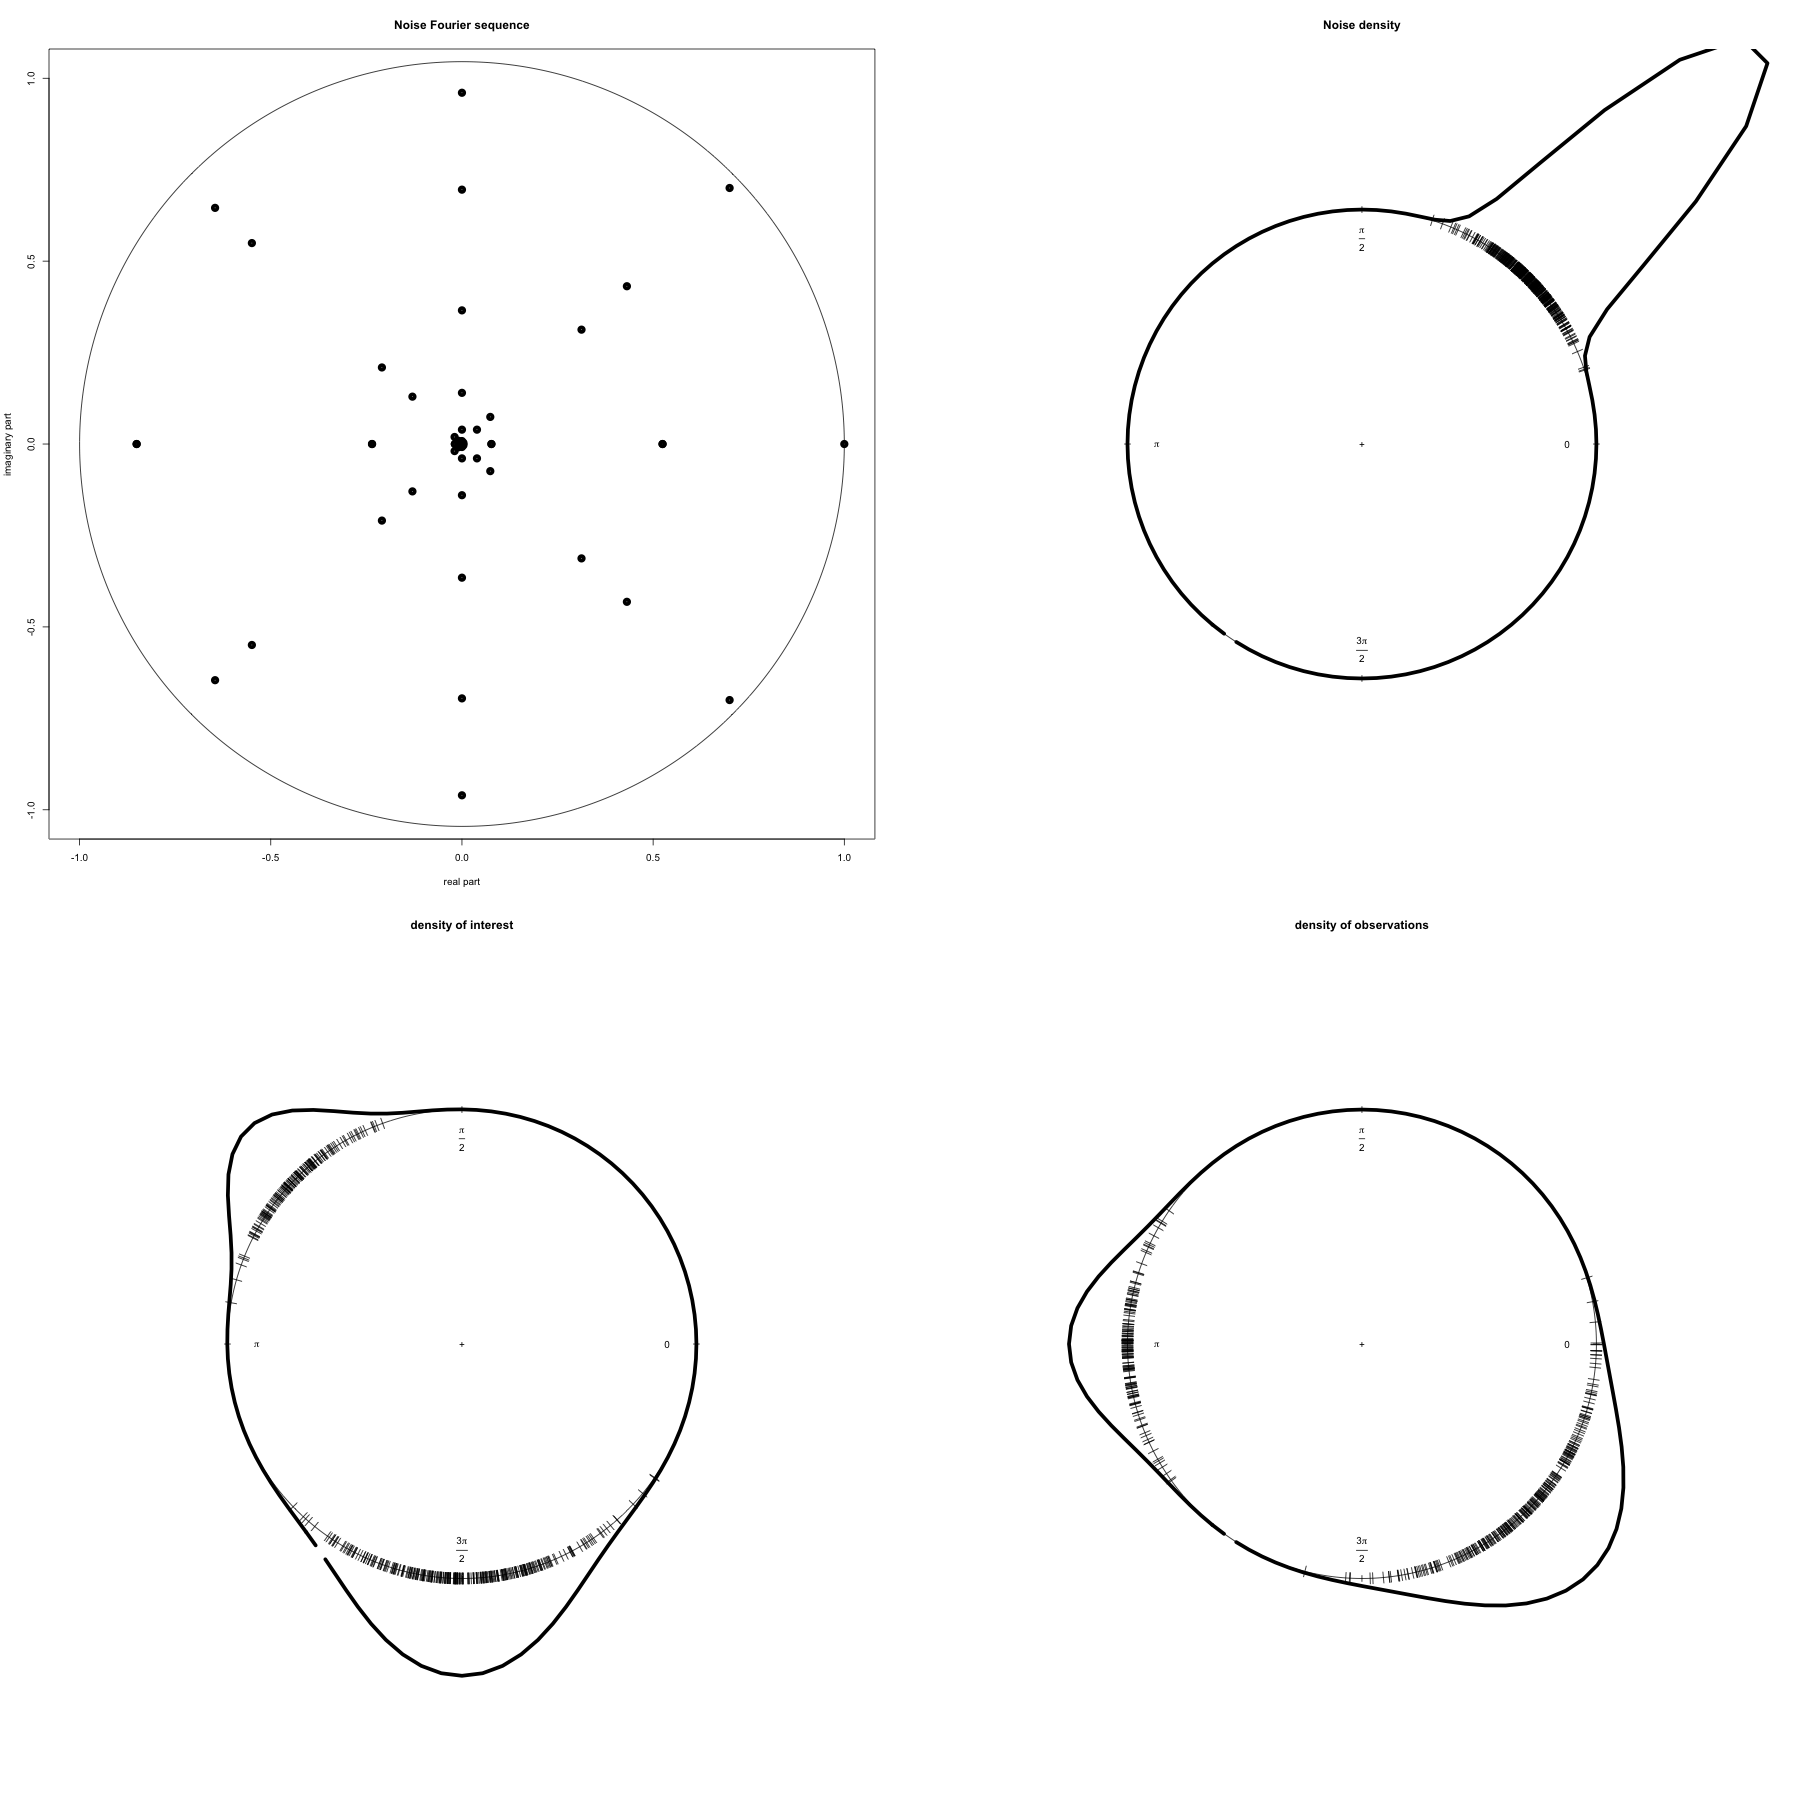
\includegraphics[width=.4\linewidth]{density/illu-deconv2/950.png} \\[\abovecaptionskip]
  \end{tabular}
  \begin{tabular}{@{}c@{}}
    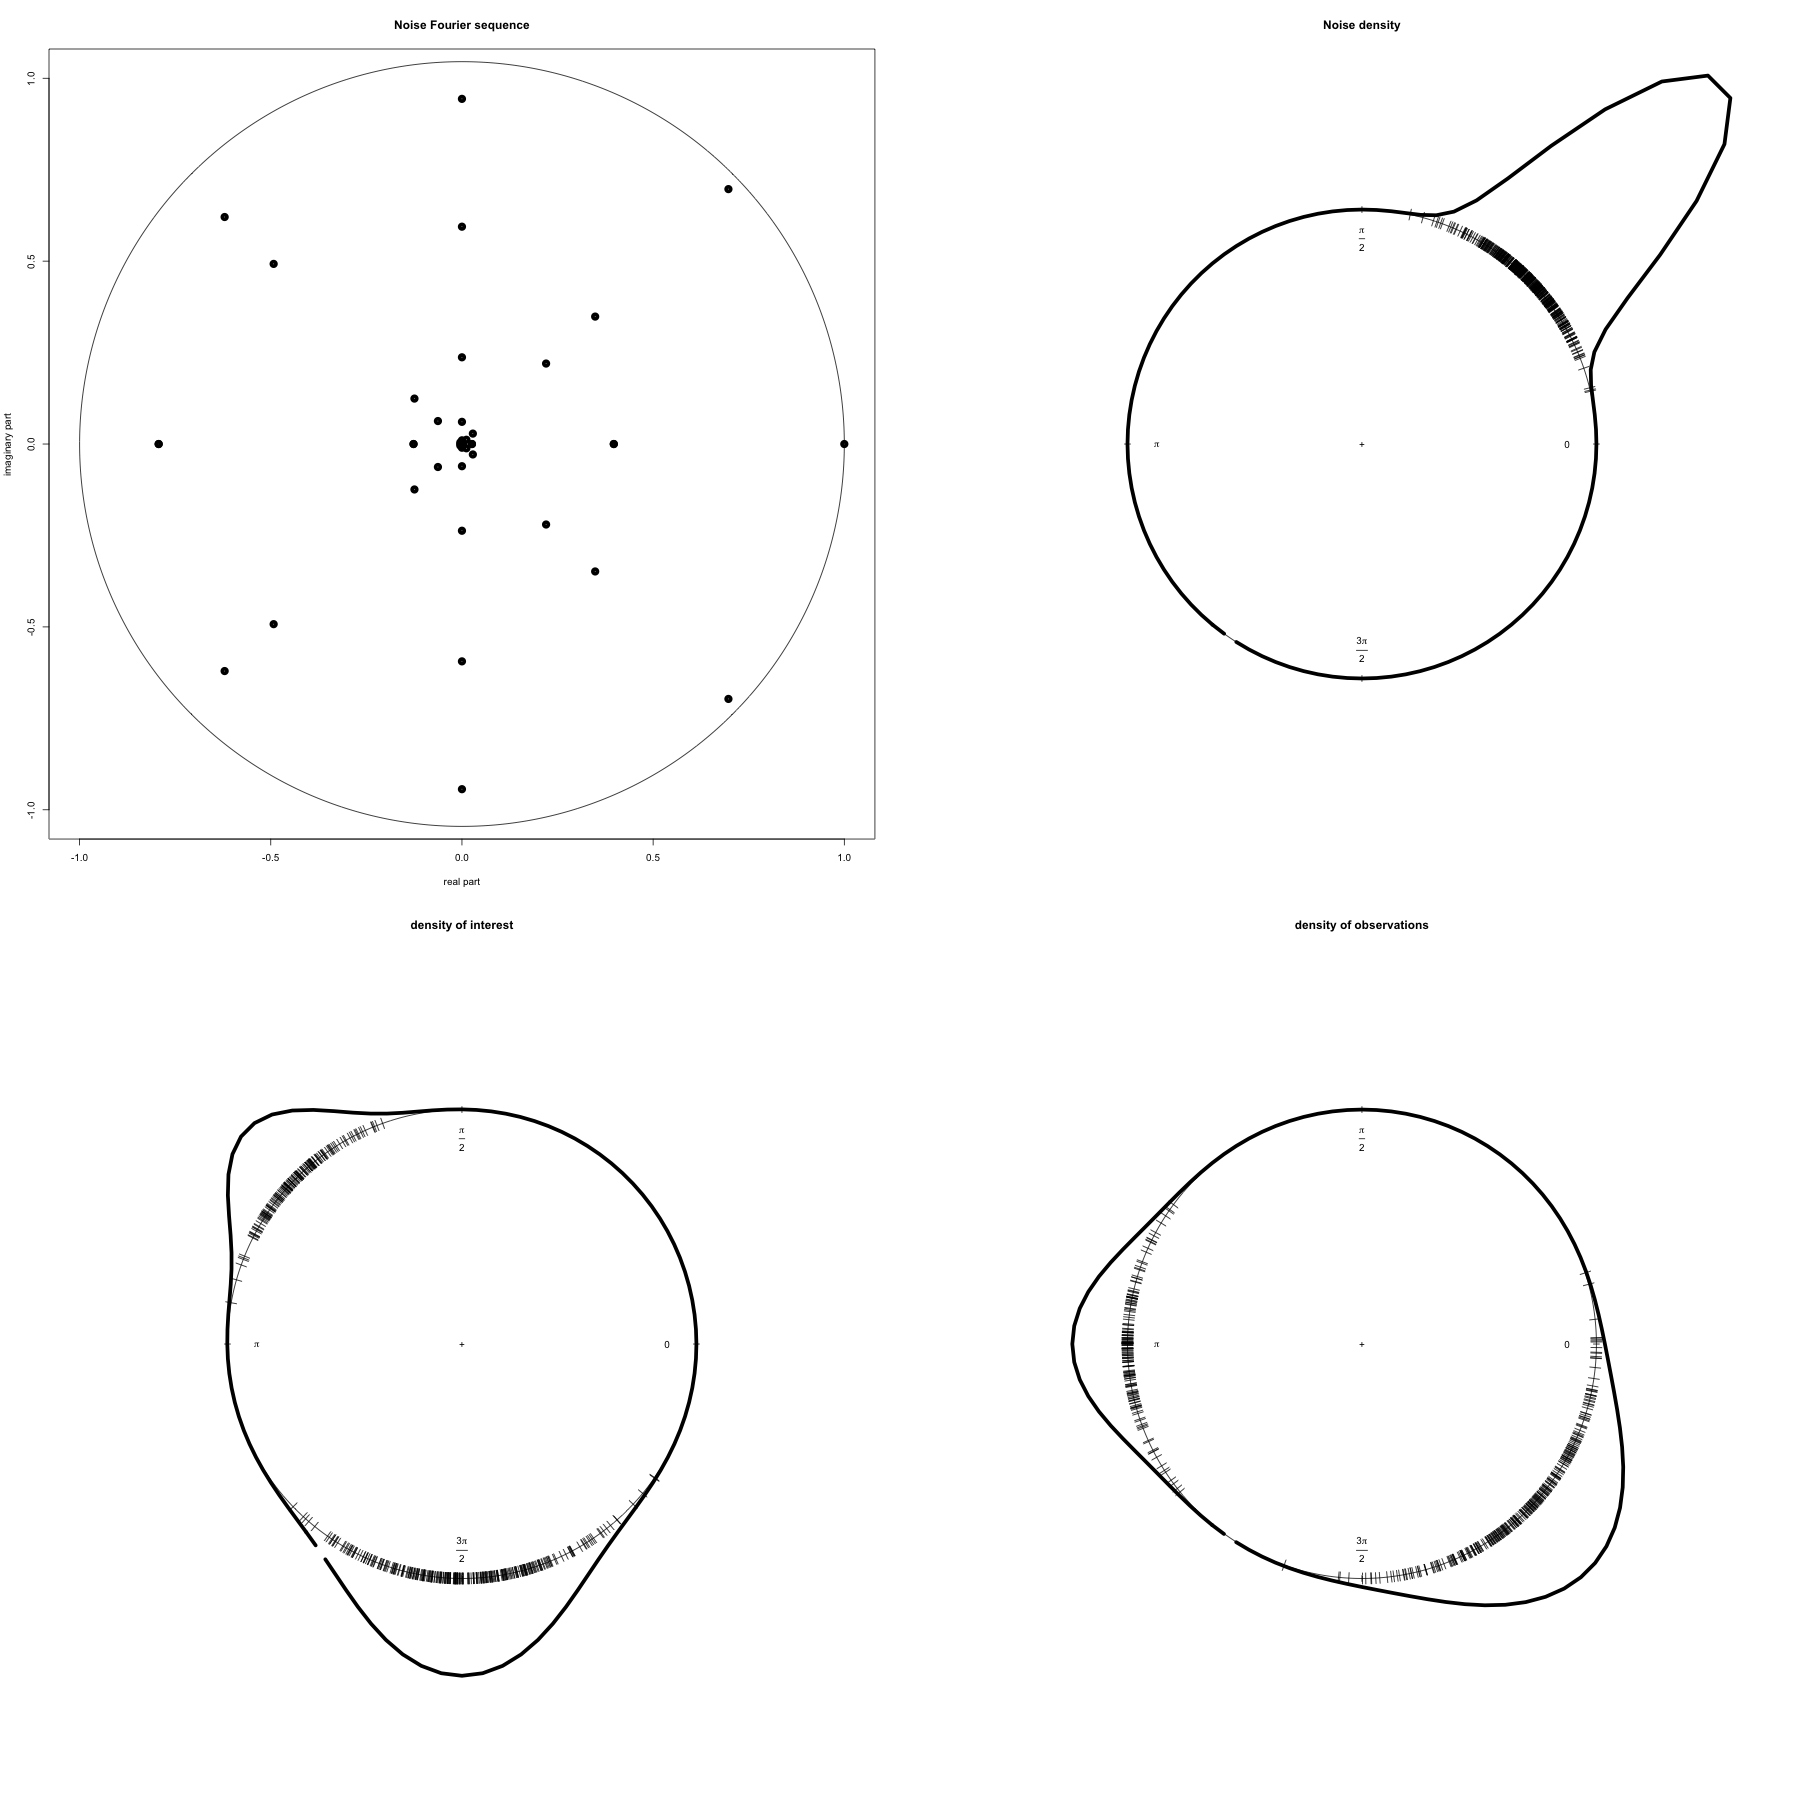
\includegraphics[width=.4\linewidth]{density/illu-deconv2/965.png} \\[\abovecaptionskip]
  \end{tabular}

  \vspace{\floatsep}

  \begin{tabular}{@{}c@{}}
    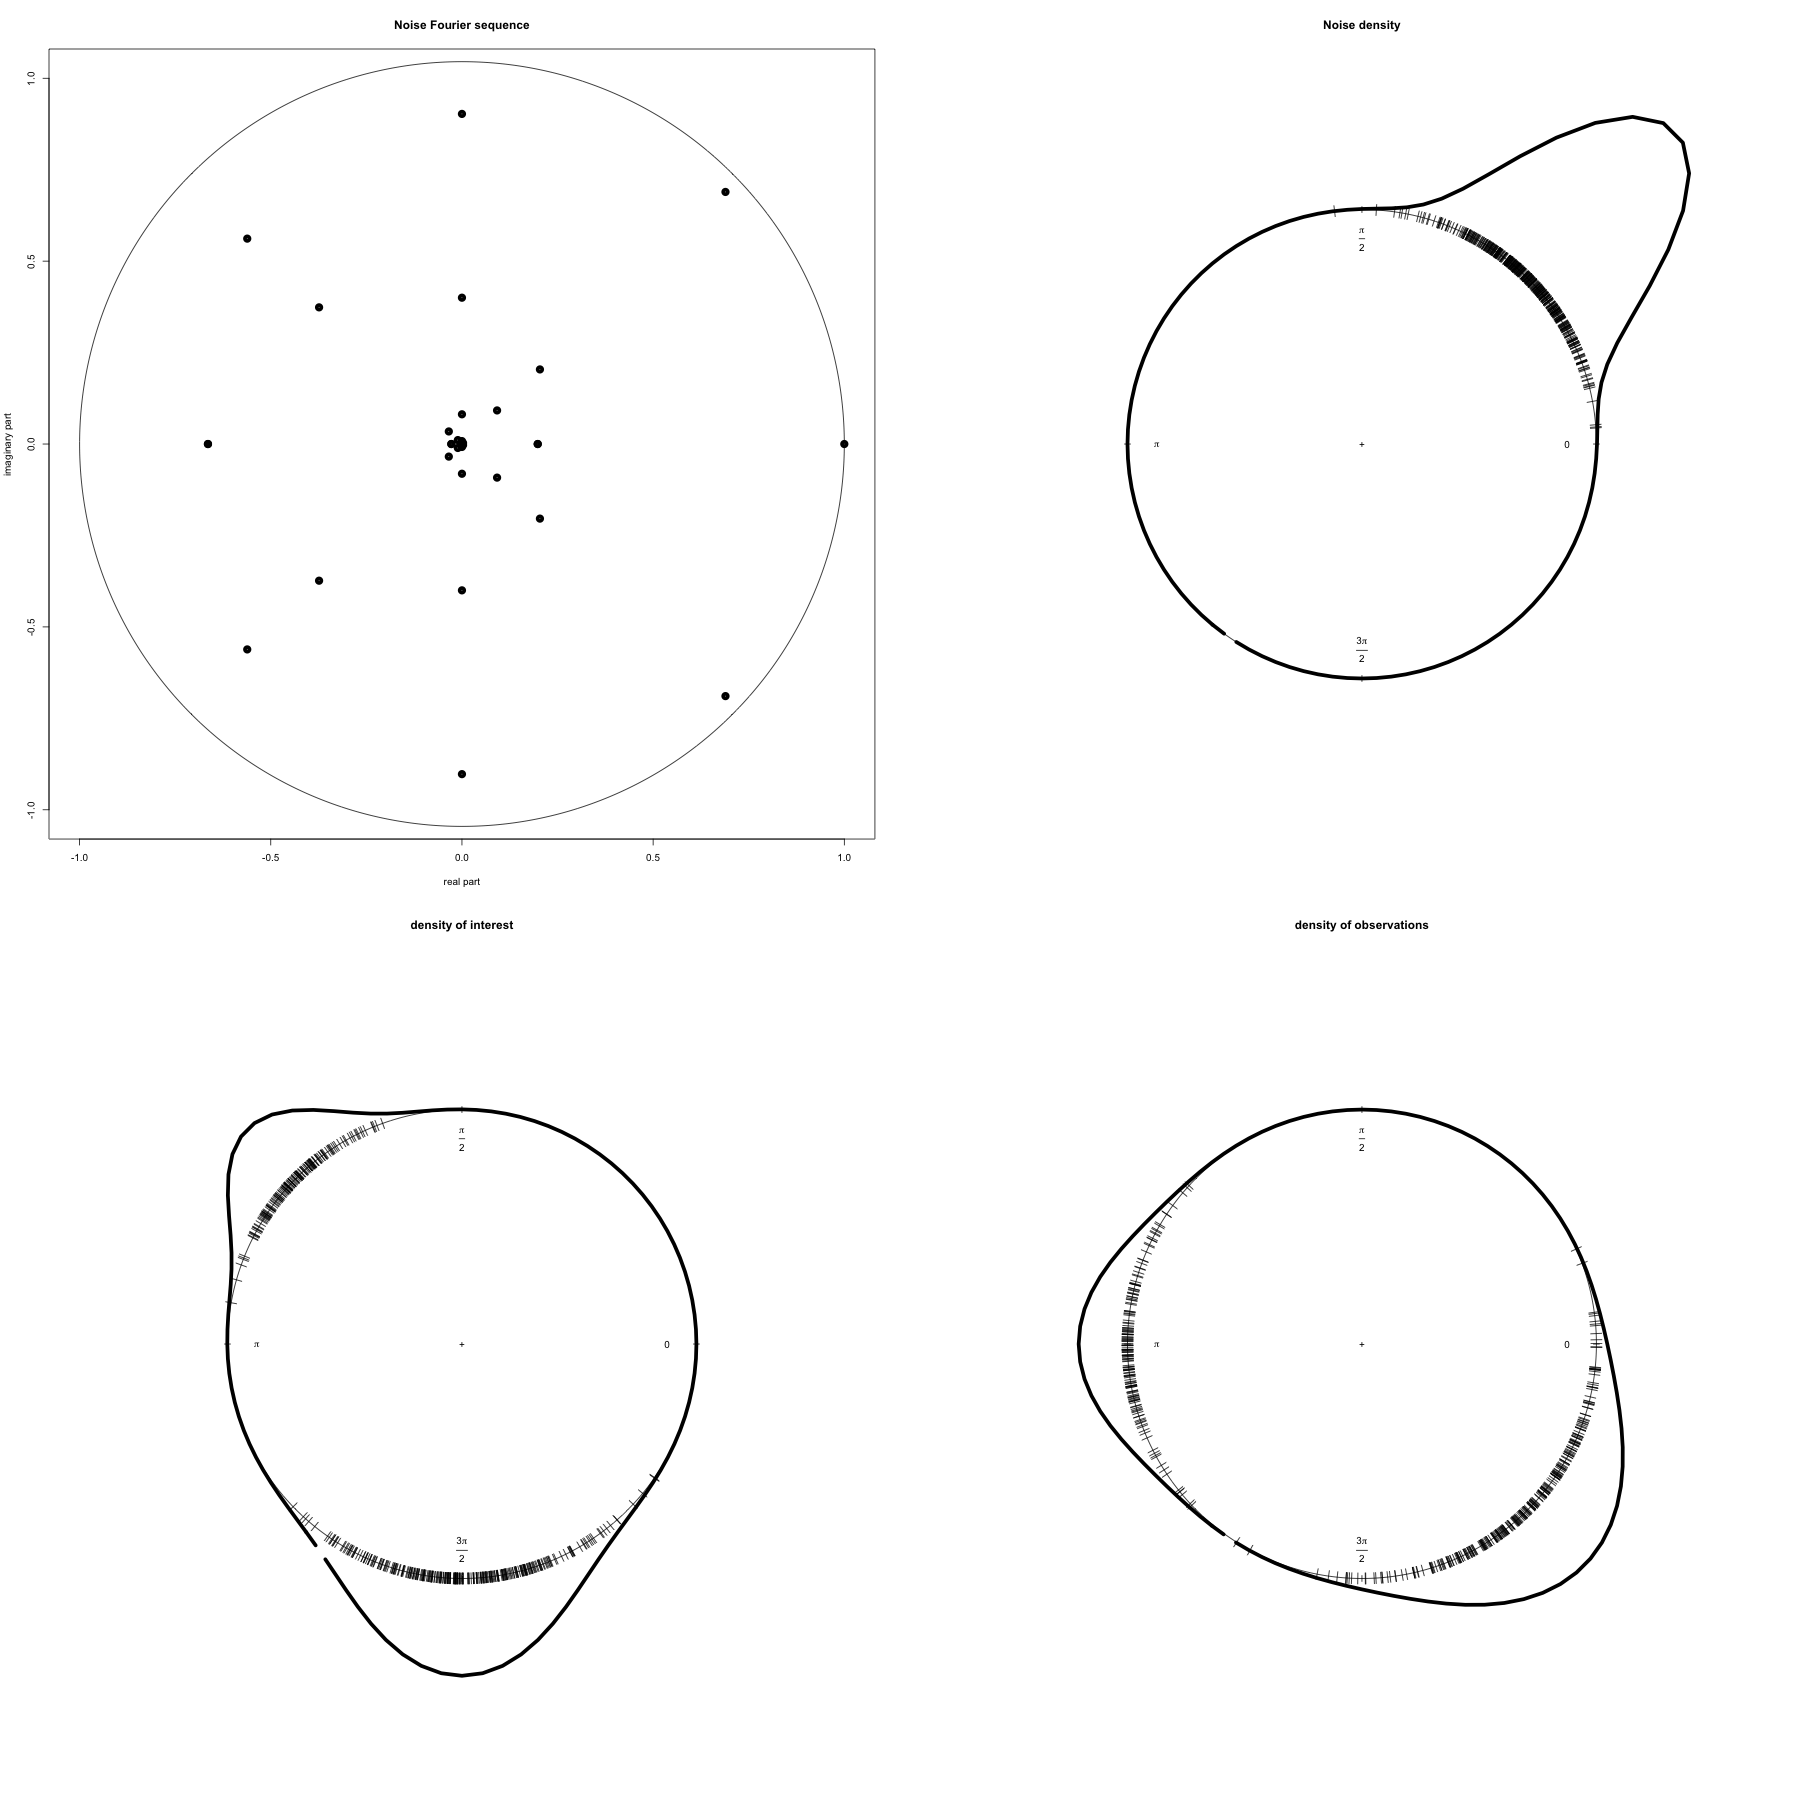
\includegraphics[width=.4\linewidth]{density/illu-deconv2/980.png} \\[\abovecaptionskip]
  \end{tabular}
  \begin{tabular}{@{}c@{}}
    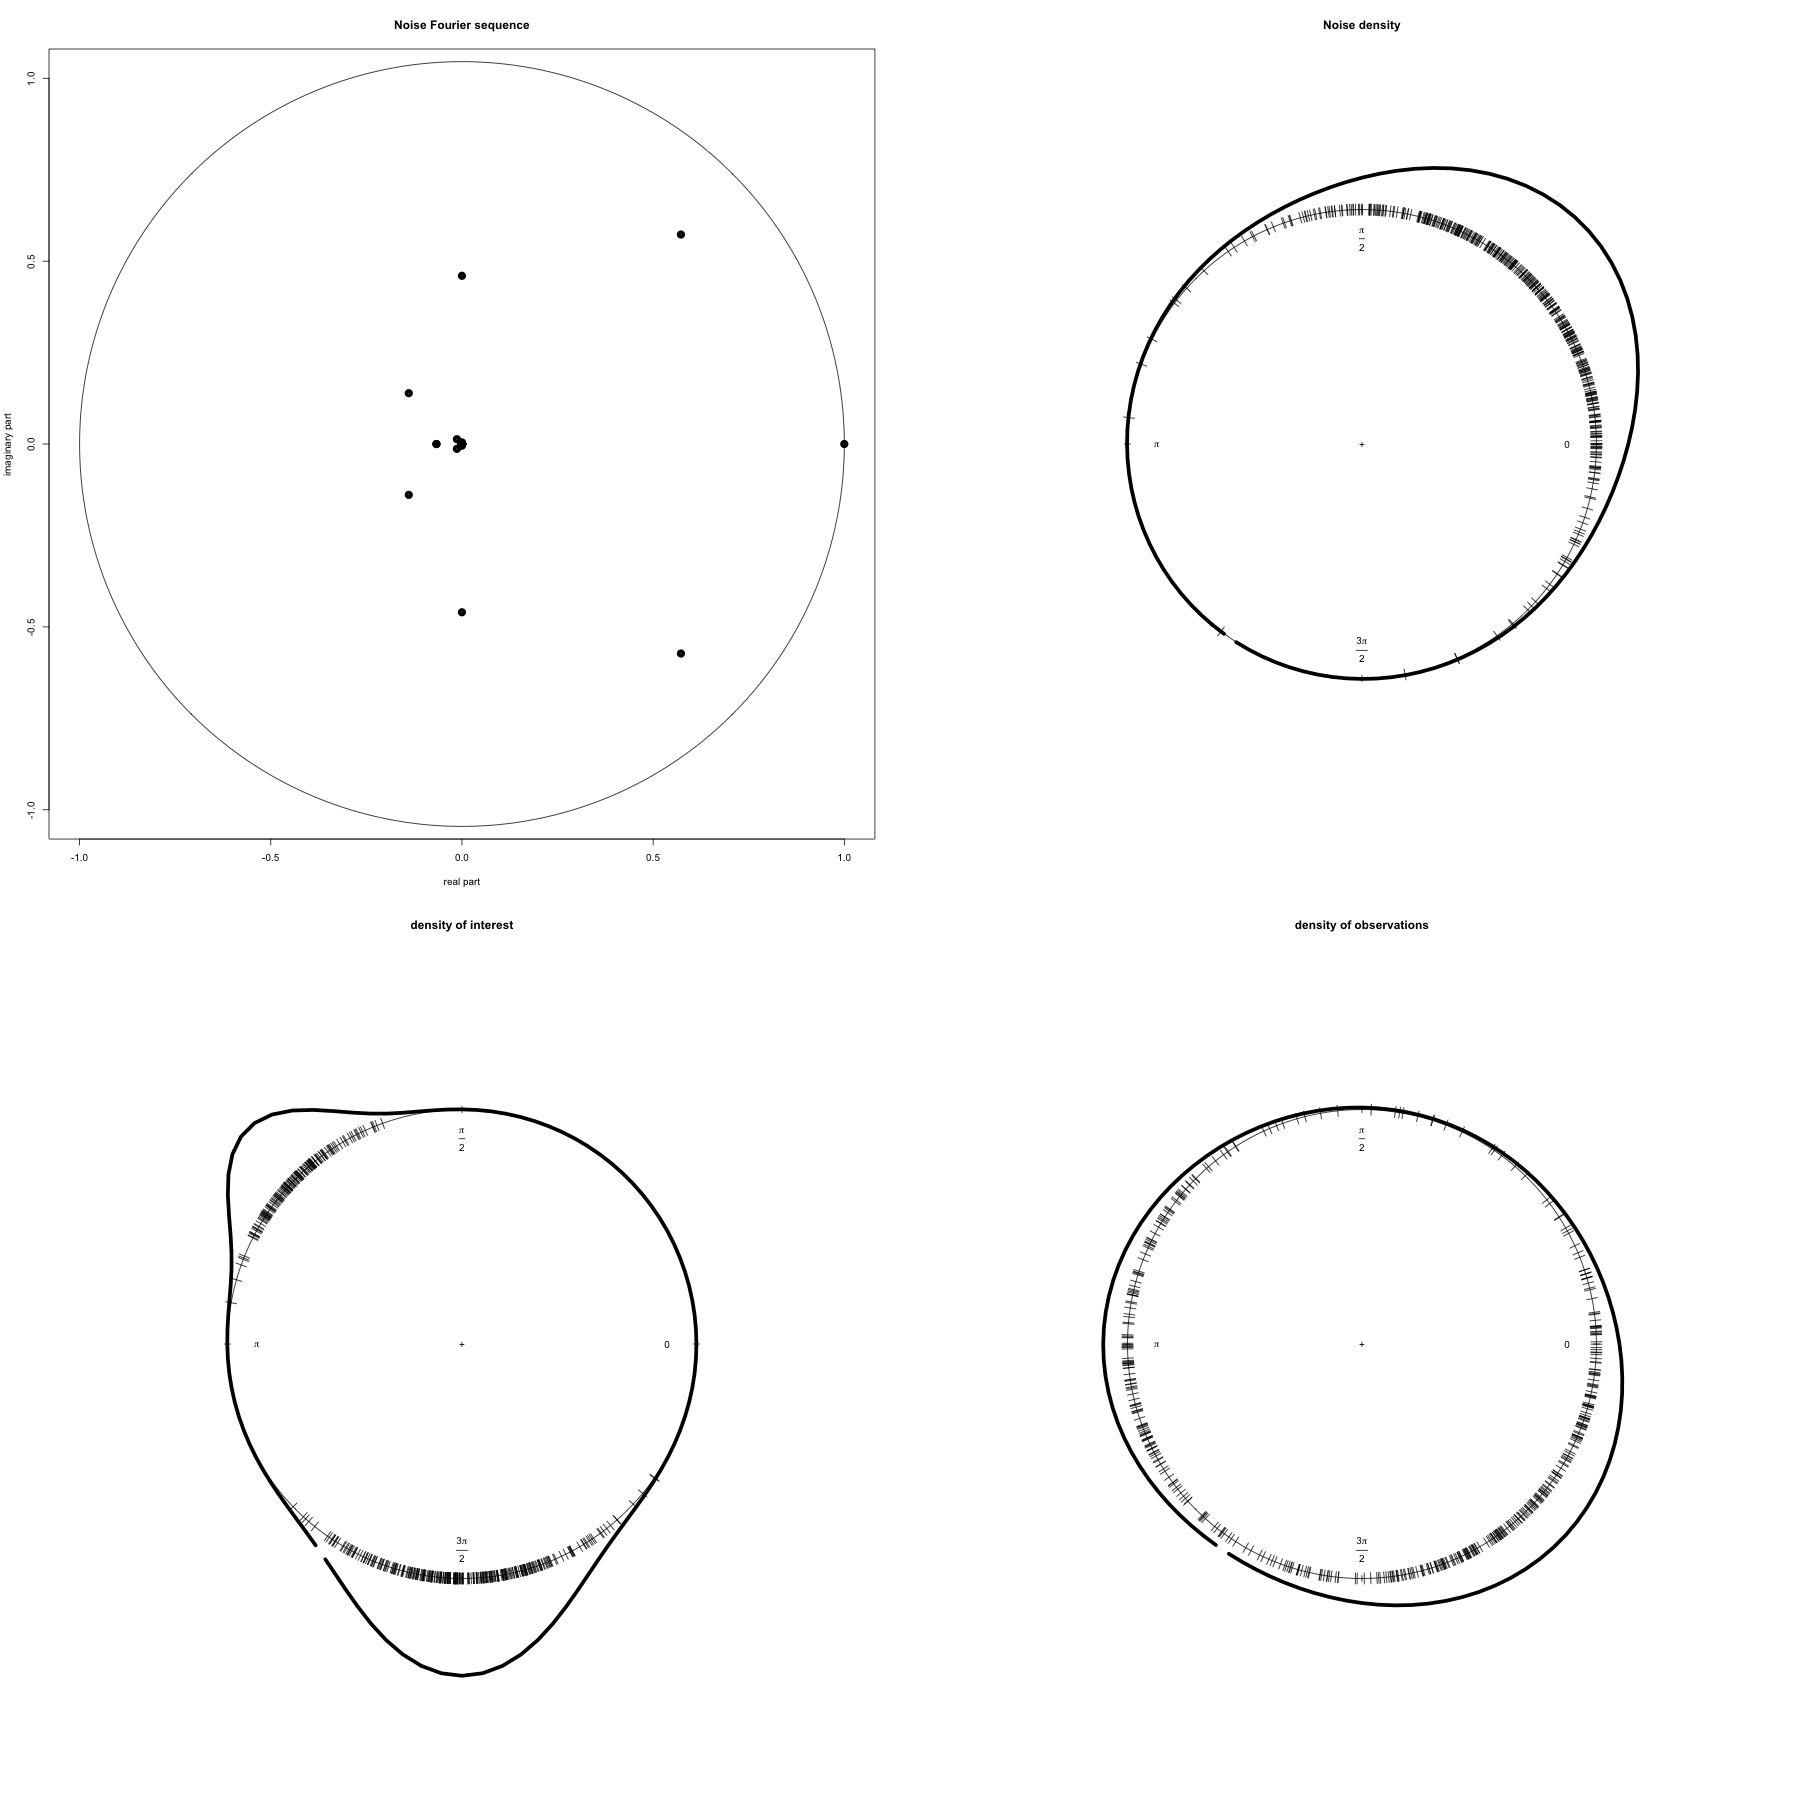
\includegraphics[width=.4\linewidth]{density/illu-deconv2/997.png} \\[\abovecaptionskip]
  \end{tabular}

  \caption{Influence of the noise density smoothness on the observation density}\label{fig:myfig}
\end{figure}

\begin{figure}
  \centering
  \begin{tabular}{@{}c@{}}
    \includegraphics[width=.4\linewidth]{density/anim-proj/1.png} \\[\abovecaptionskip]
  \end{tabular}
  \begin{tabular}{@{}c@{}}
    \includegraphics[width=.4\linewidth]{density/anim-proj/8.png} \\[\abovecaptionskip]
  \end{tabular}

  \vspace{\floatsep}

  \begin{tabular}{@{}c@{}}
    \includegraphics[width=.4\linewidth]{density/anim-proj/16.png} \\[\abovecaptionskip]
  \end{tabular}
  \begin{tabular}{@{}c@{}}
    \includegraphics[width=.4\linewidth]{density/anim-proj/24.png} \\[\abovecaptionskip]
  \end{tabular}

  \caption{Influence of the threshold parameter choice on the estimation in the direct problem case}\label{circ:proj:direct}
\end{figure}

\begin{figure}
  \centering
  \begin{tabular}{@{}c@{}}
    \includegraphics[width=.4\linewidth]{density/anim-proj-expo/1.png} \\[\abovecaptionskip]
  \end{tabular}
  \begin{tabular}{@{}c@{}}
    \includegraphics[width=.4\linewidth]{density/anim-proj-expo/8.png} \\[\abovecaptionskip]
  \end{tabular}

  \vspace{\floatsep}

  \begin{tabular}{@{}c@{}}
    \includegraphics[width=.4\linewidth]{density/anim-proj-expo/16.png} \\[\abovecaptionskip]
  \end{tabular}
  \begin{tabular}{@{}c@{}}
    \includegraphics[width=.4\linewidth]{density/anim-proj-expo/24.png} \\[\abovecaptionskip]
  \end{tabular}

  \caption{Influence of the threshold parameter choice on the estimation in the severely ill-posed problem case}\label{circ:proj:expo}
\end{figure}

%\begin{figure}
%\centering
%\begin{subfigure}{.4\textwidth}
%  \centering
%  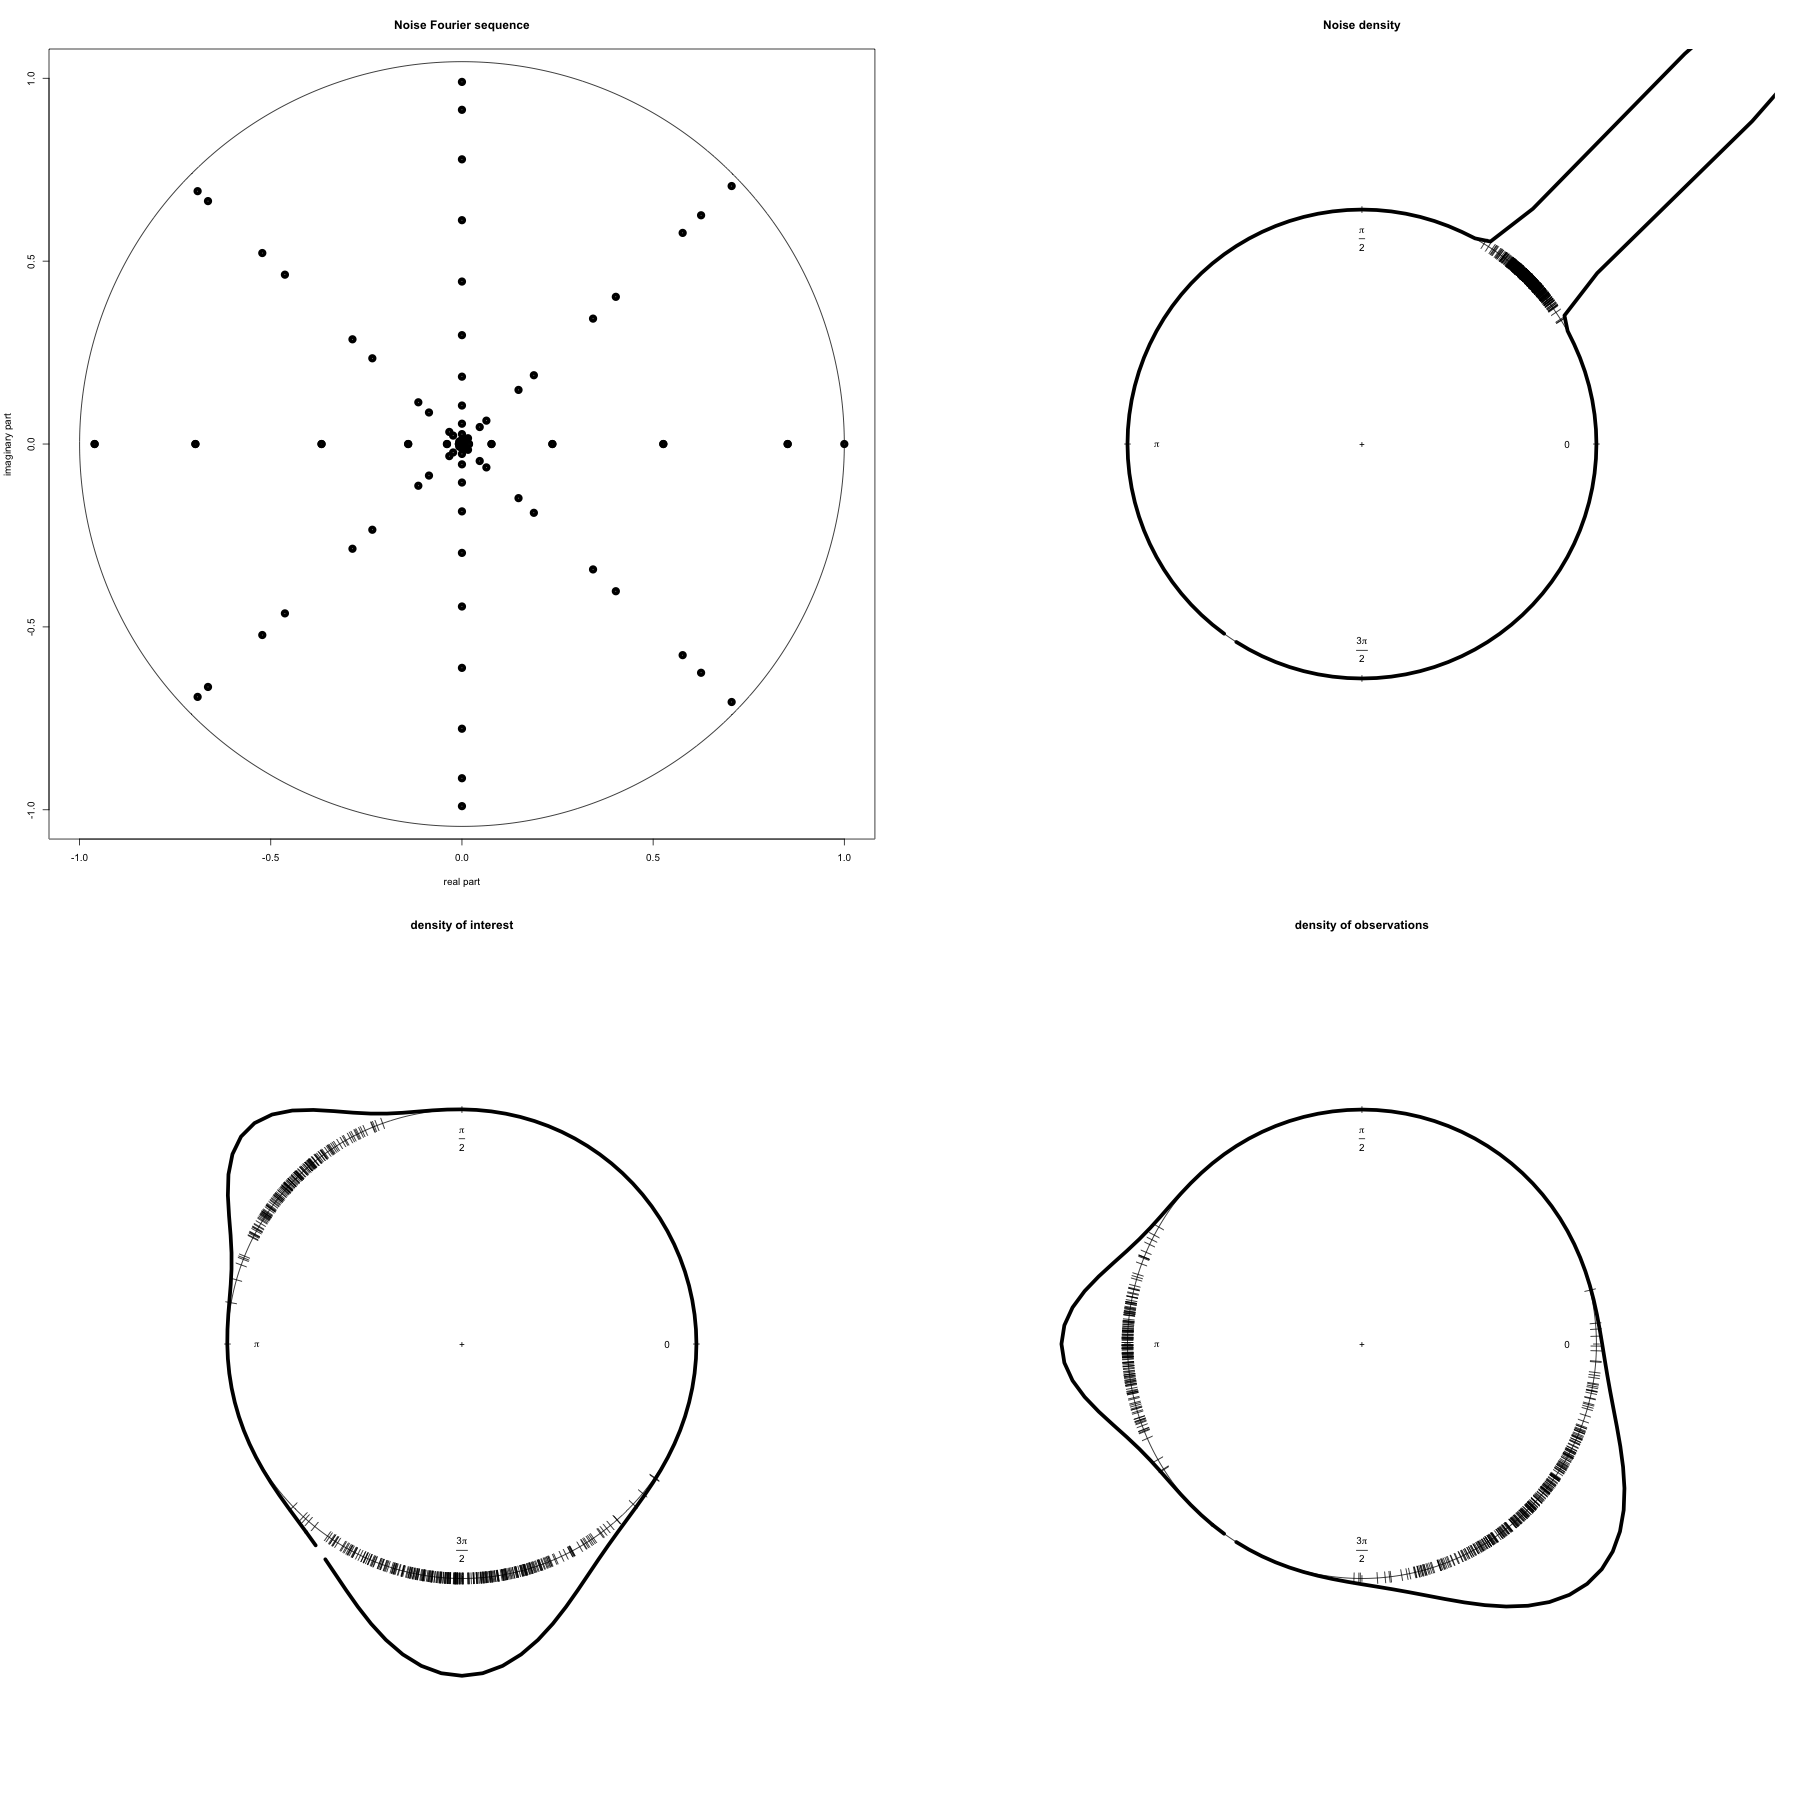
\includegraphics[width=1.\linewidth]{density/illu-deconv2/800.png}
%  \caption{$\theta^{\circ}$ polynomial and $\lambda$ polynomial}
%  \label{fig3:sub1}
%\end{subfigure}%
%\begin{subfigure}{.4\textwidth}
%  \centering
%  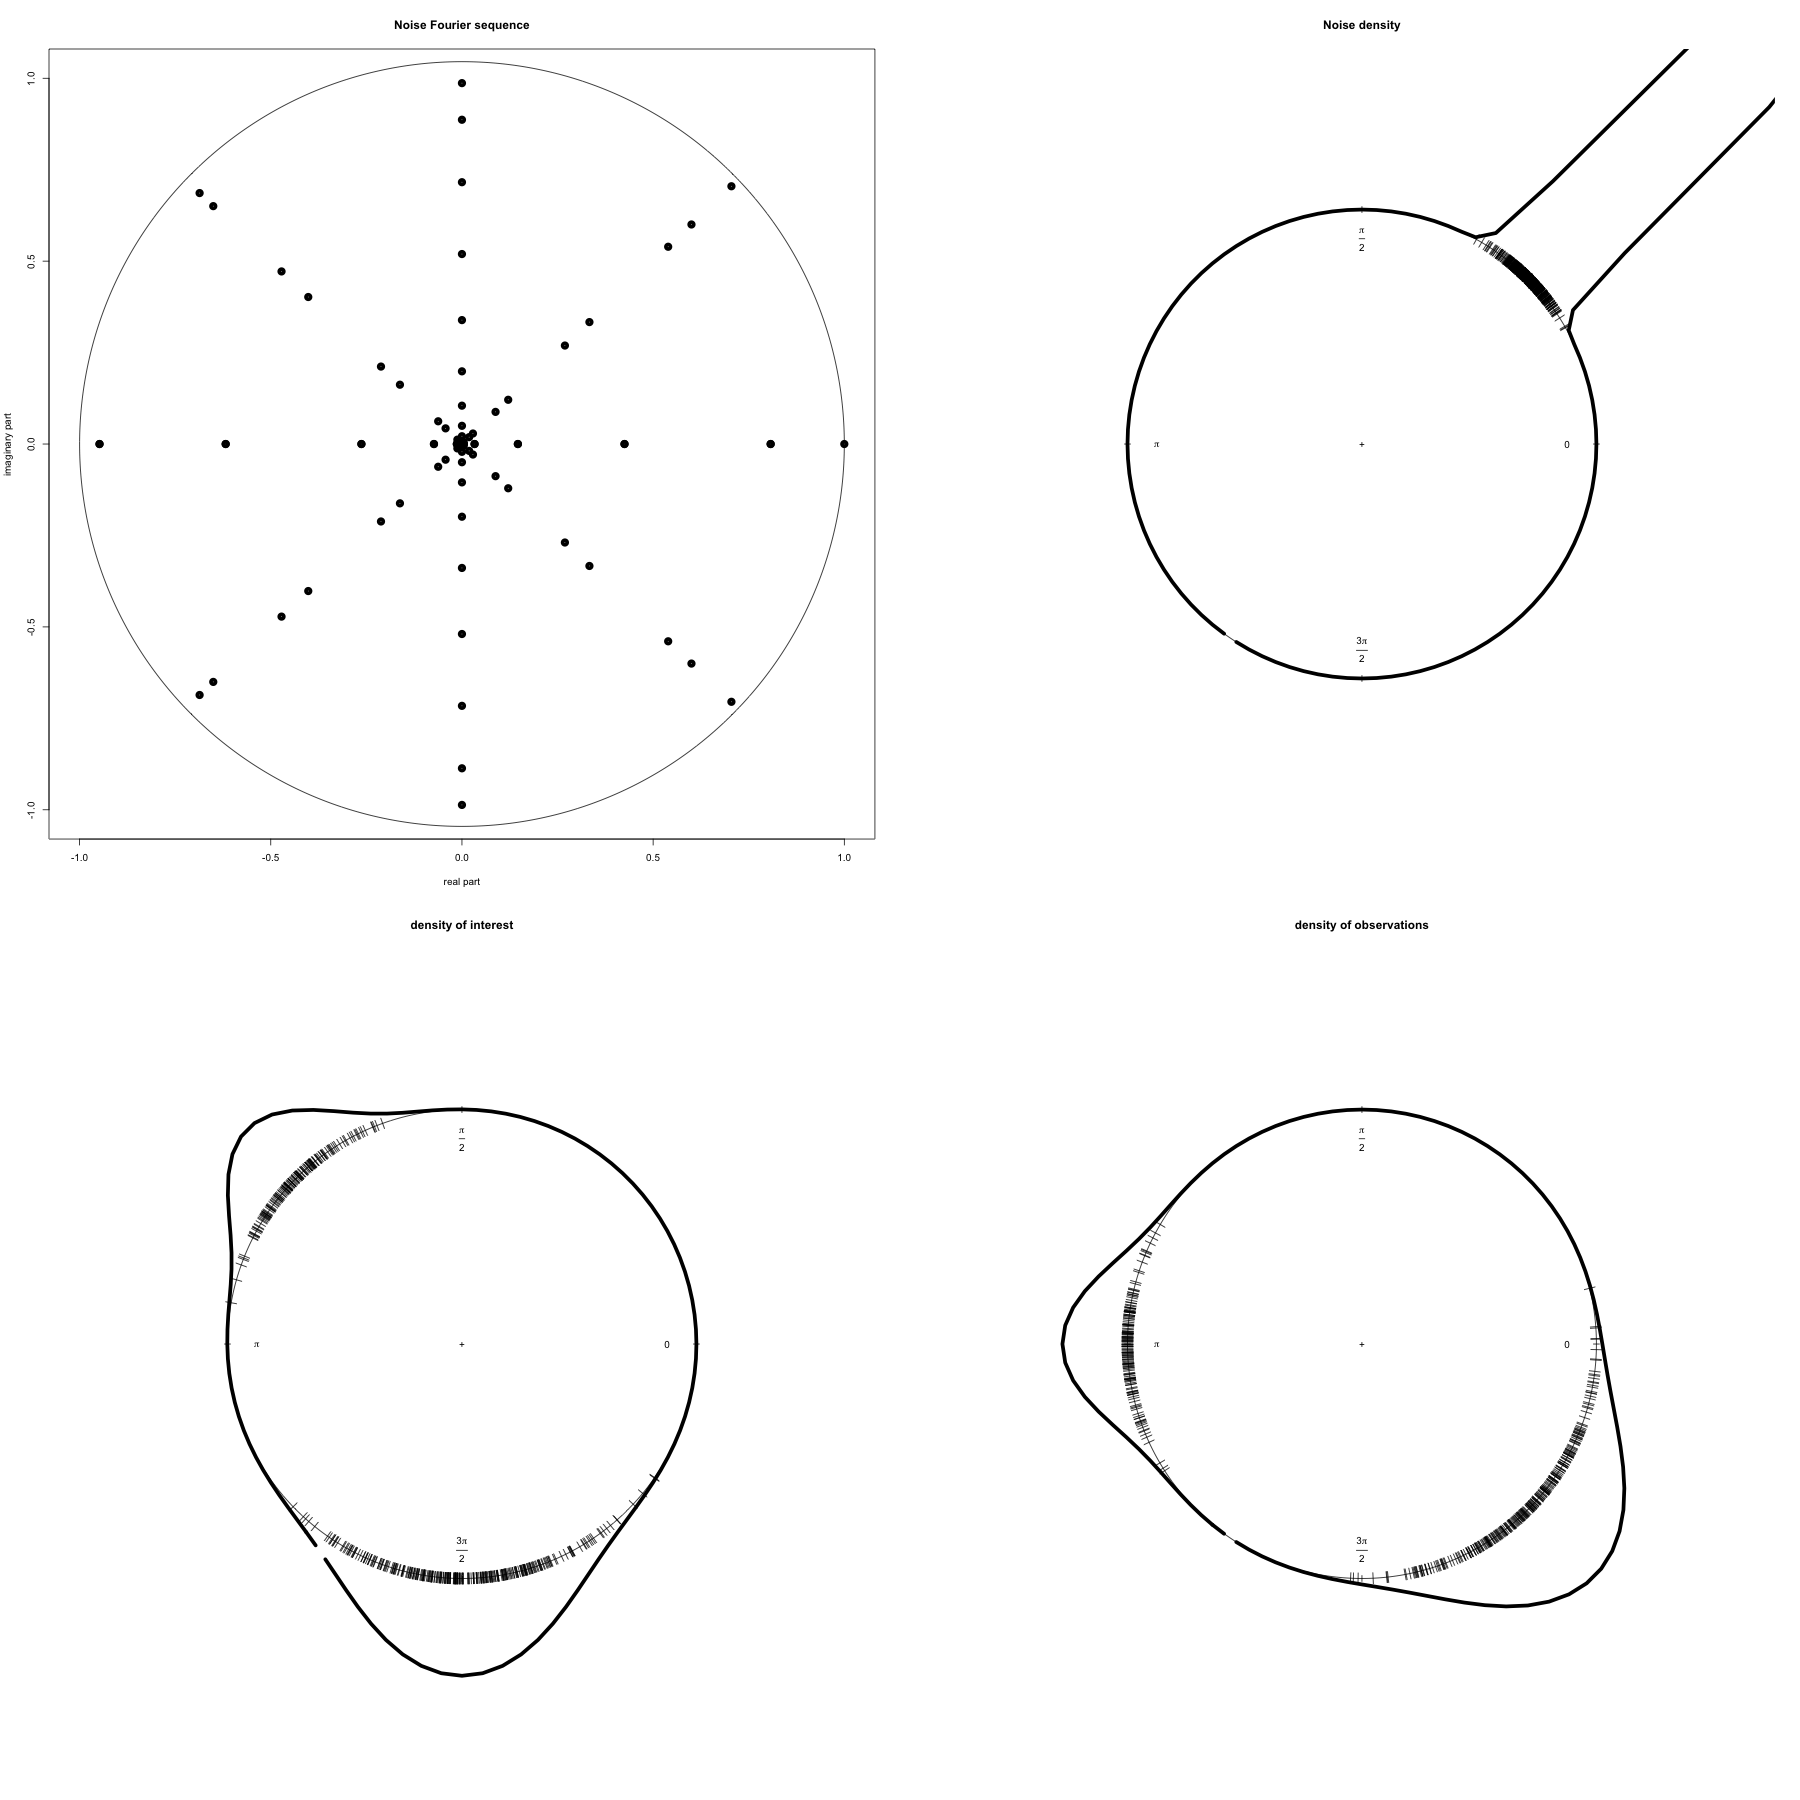
\includegraphics[width=1.\linewidth]{density/illu-deconv2/850.png}
%  \caption{$\theta^{\circ}$ polynomial and $\lambda$ exponential}
%  \label{fig3:sub2}
%\end{subfigure}
%\begin{subfigure}{.4\textwidth}
%  \centering
%  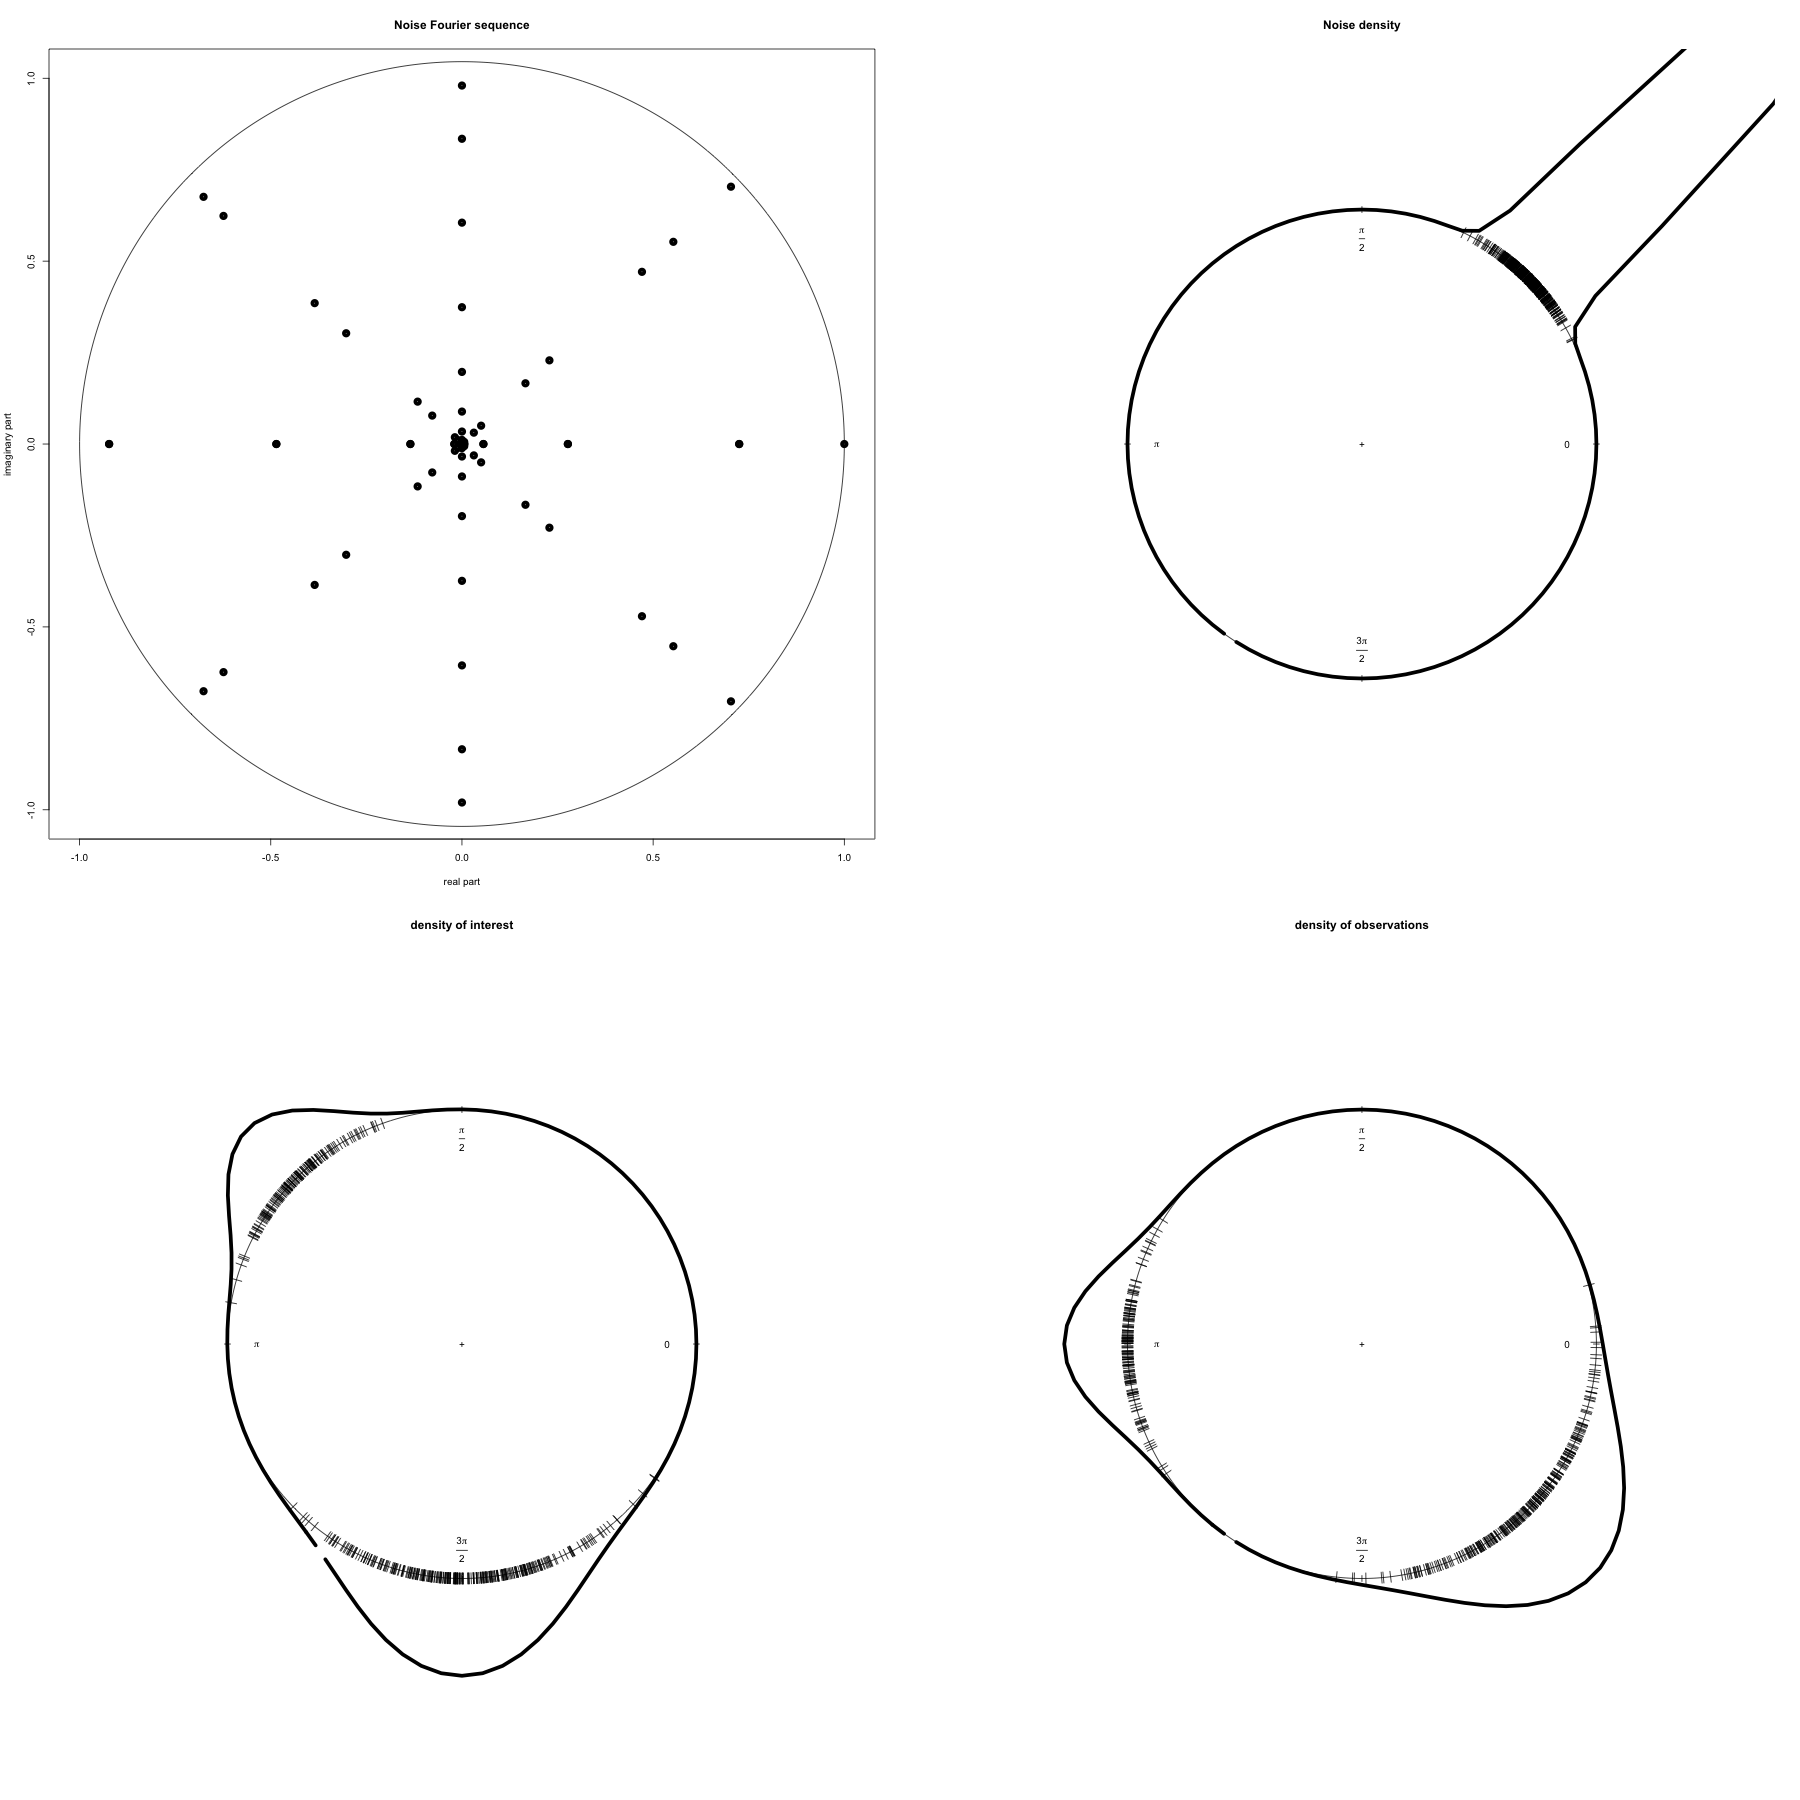
\includegraphics[width=1.\linewidth]{density/illu-deconv2/900.png}
%  \caption{$\theta^{\circ}$ polynomial and $\lambda$ exponential}
%  \label{fig3:sub3}
%\end{subfigure}
%\begin{subfigure}{.4\textwidth}
%  \centering
%  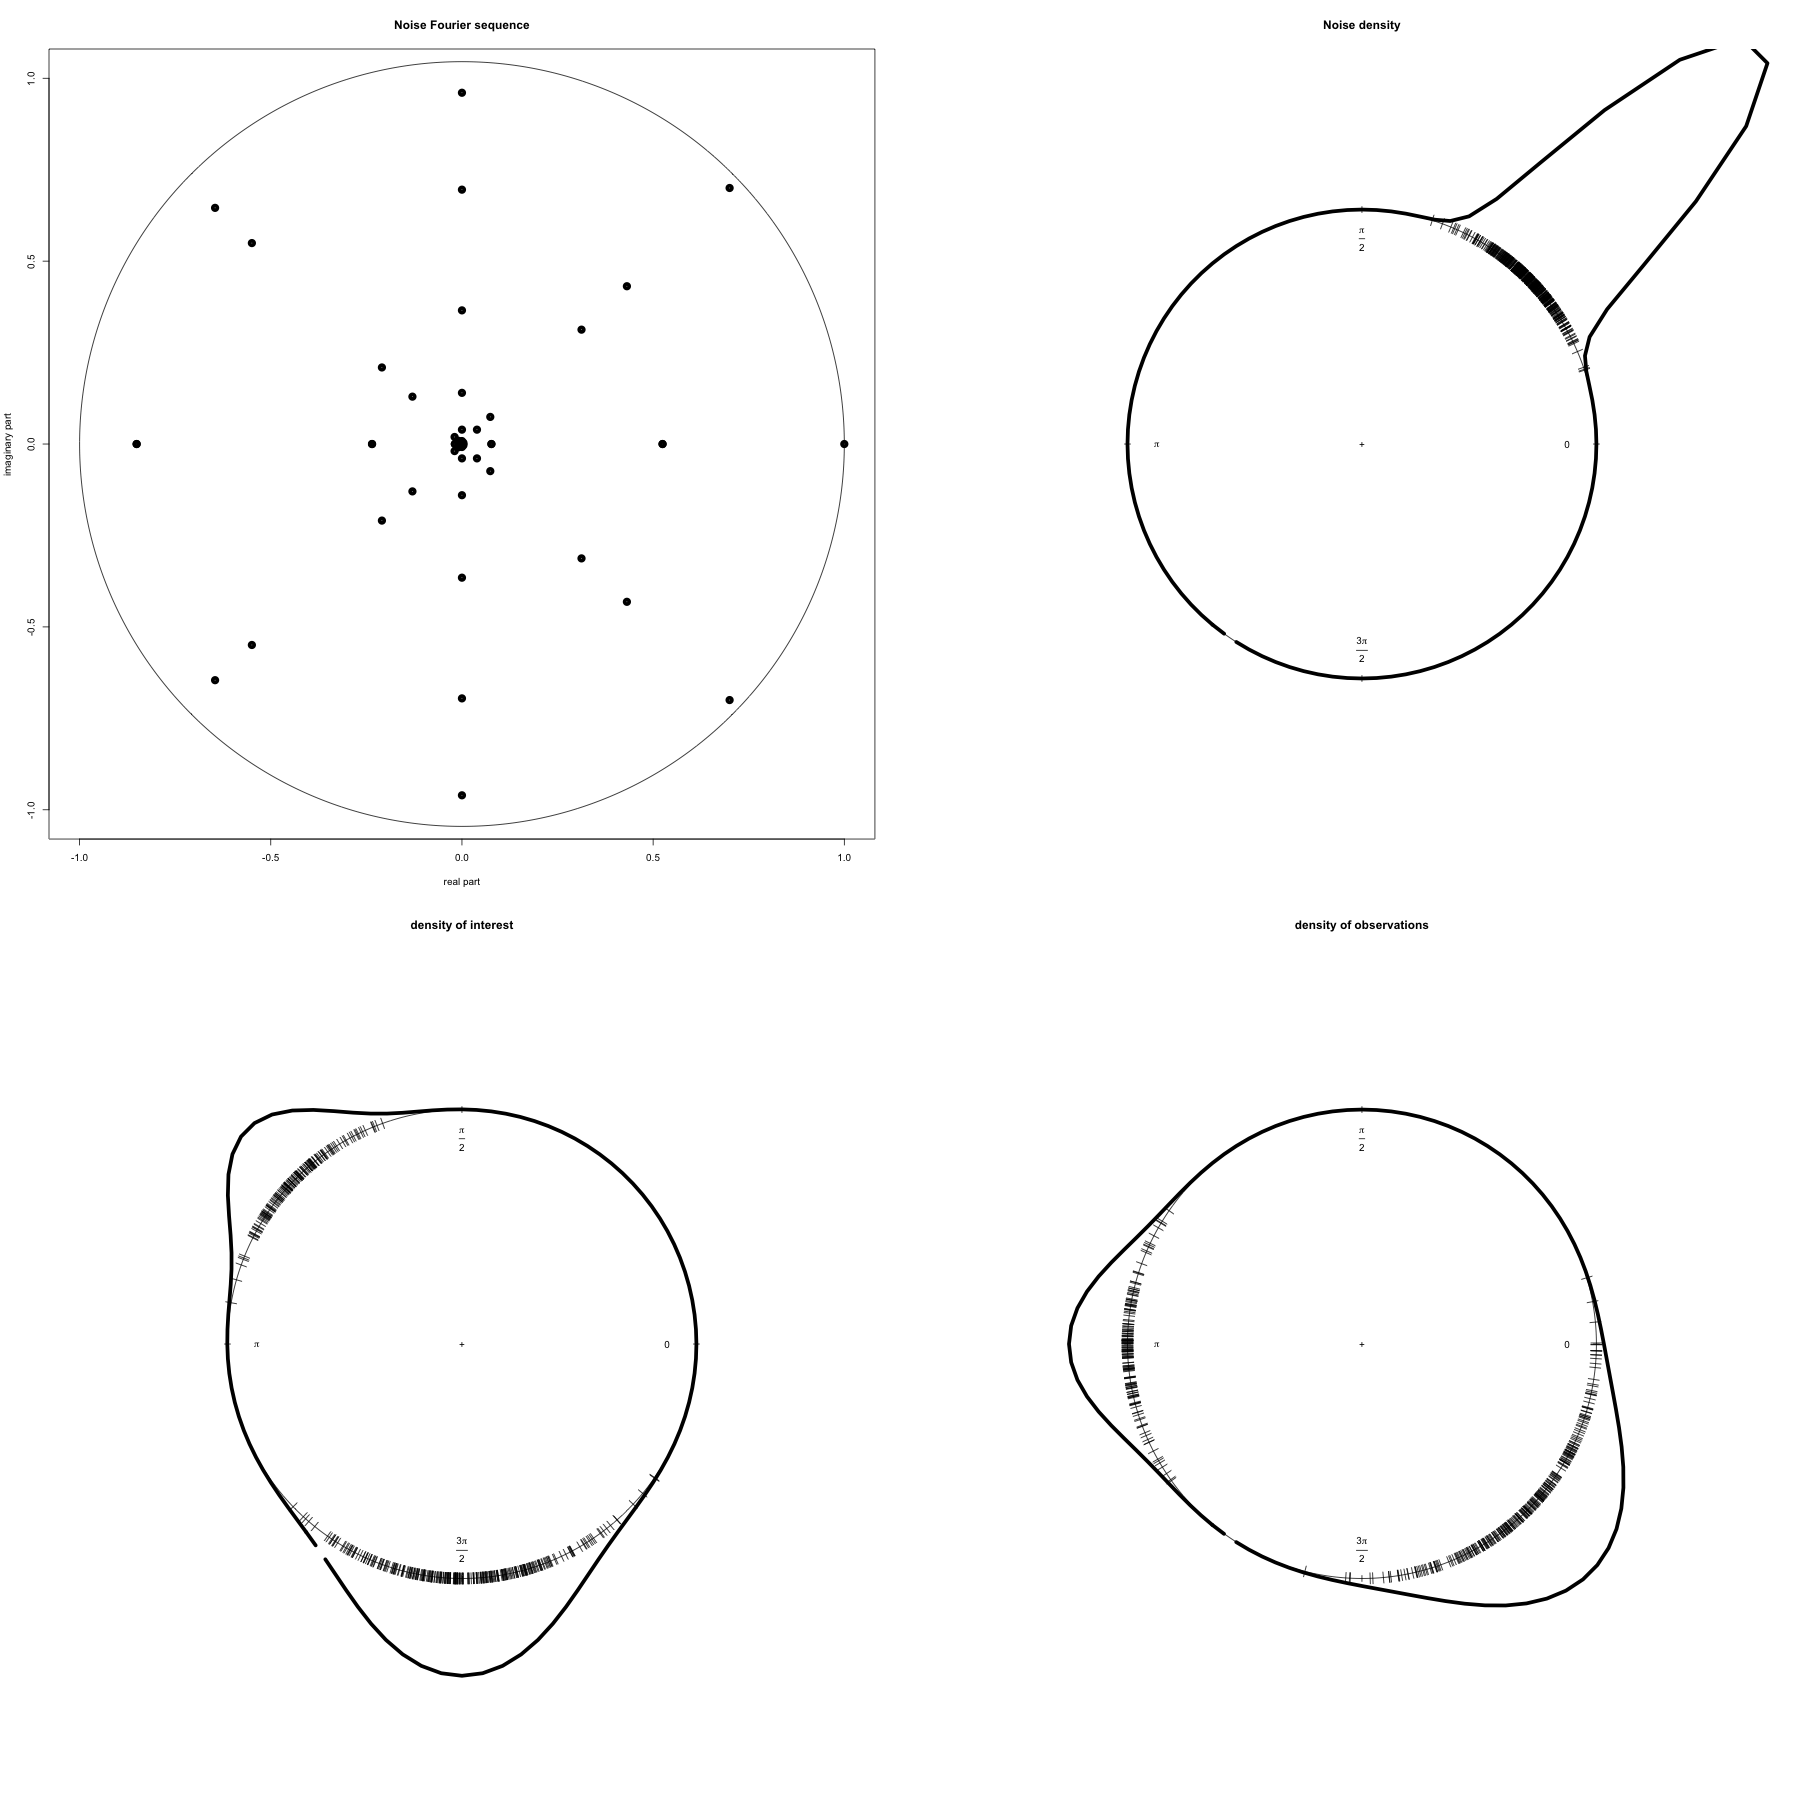
\includegraphics[width=1.\linewidth]{density/illu-deconv2/950.png}
%  \caption{$\theta^{\circ}$ polynomial and $\lambda$ exponential}
%  \label{fig3:sub4}
%\end{subfigure}
%\begin{subfigure}{.4\textwidth}
%  \centering
%  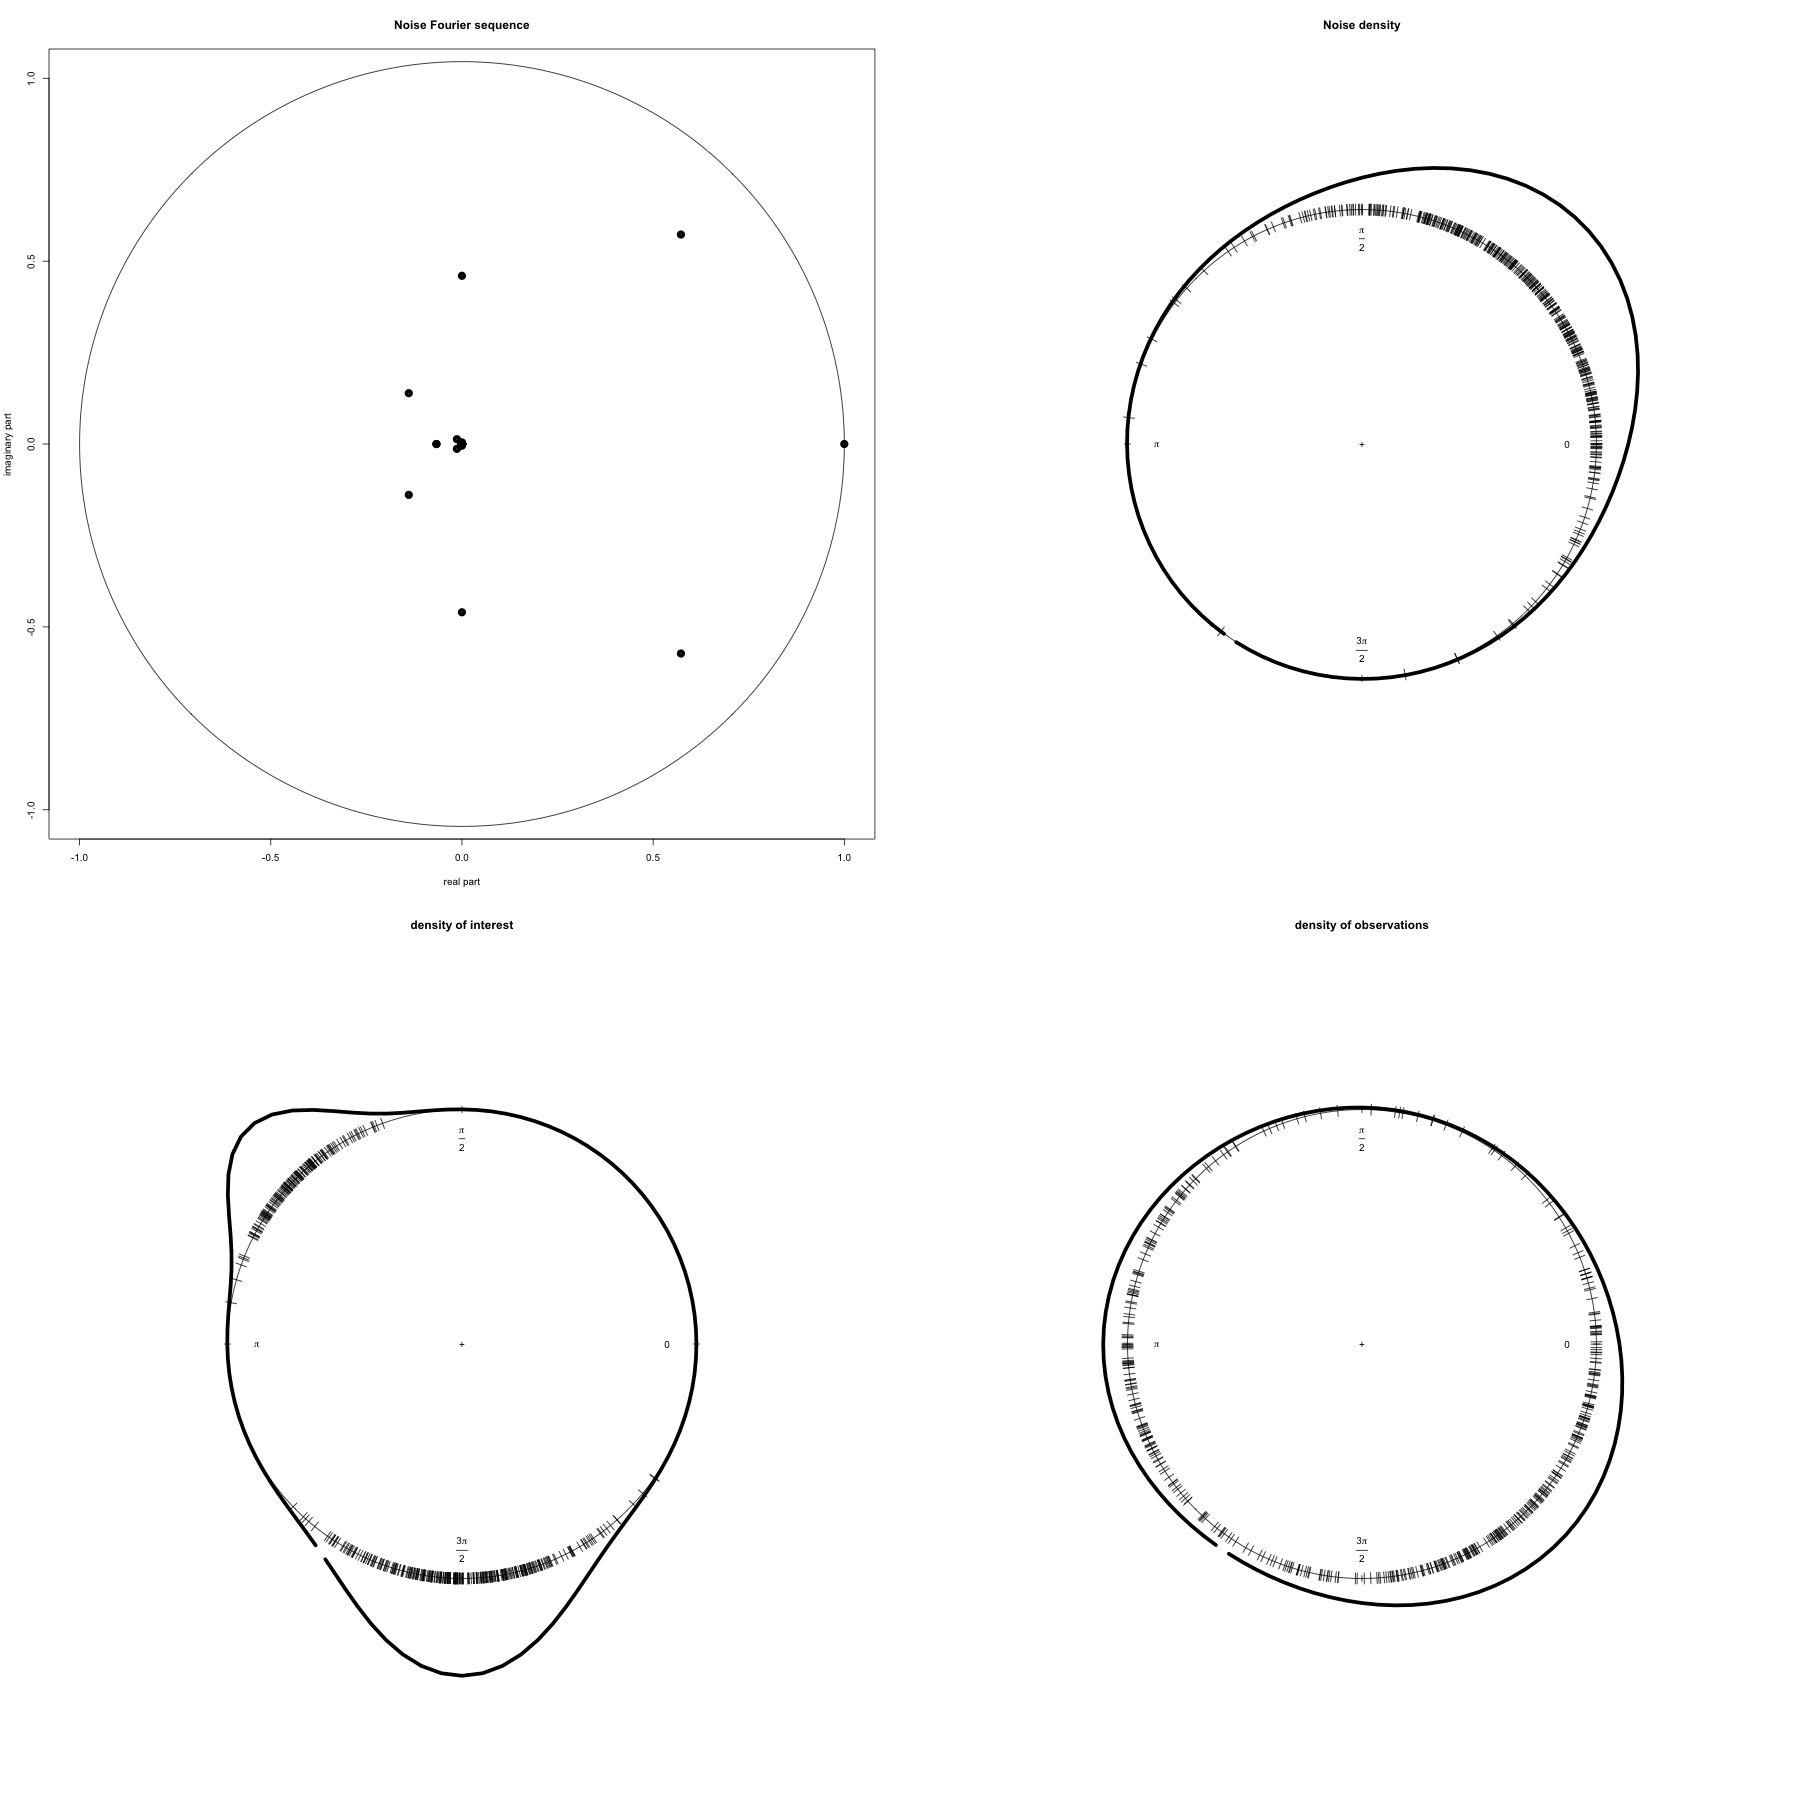
\includegraphics[width=1.\linewidth]{density/illu-deconv2/997.png}
%  \caption{$\theta^{\circ}$ polynomial and $\lambda$ exponential}
%  \label{fig3:sub5}
%\end{subfigure}
%\caption{Estimated median of the quadratic error of the estimator given by the posterior mean for different classes of $\theta^{\circ}$ and $\lambda$ with $\theta^{\times} \equiv 0$ and $s \equiv 1$.}
%\label{EQM}
%\end{figure}

\subsection{Known noise density, independent observations process}
% ....................................................................
% Oracle optimality known error density
% ....................................................................
\begin{te}
We place ourselves under \nref{AS_INTRO_DATA_KNOWN} and \nref{AS_INTRO_DATA_INDEPENDENT}.
We hence observe an \iid $\ssY$-sample $\rY_1,\dotsc,\rY_{\ssY}$ from $g = f \star h$.
Given an estimator $\hxdf[]$ of $\xdf\in\lp[2]$ based on the observations we measure its accuracy by a quadratic risk, that is, $\E\Vnormlp{\hxdf[]-\xdf}^2$.
Keep in mind that throughout the thesis we assume that $ \vert \fedf[(s)] \vert >0$ holds for all $s\in\Zz$.
Considering $\Lambda=\Nsuite{\iSv[s]}$ with $\iSv[s]:= \vert \fedf[(s)] \vert ^{-2}$ for $s\in\Nz$, we set $\miSv=\max\set{\iSv[s],s\in\nset{1,\Di}}$ and $\oiSv=\tfrac{1}{\Di}\sum_{s=1}^{\Di}\iSv[s]$.

Notice that due to $\E[\Vert \theta_{n} - \theta^{\circ} \Vert_{l^{2}}^{2}] + n^{-1} \Vert \theta^{\circ}_{\underline{0}} \Vert_{l_{2}}^{2} = n^{-1} \sum_{-m \leq s \leq m} \Lambda(s) + \Vert \theta^{\circ}_{\underline{0}} \Vert_{l^{2}}^{2}(1 + n^{-1})\b_{m}^{2}(\theta^{\circ})$
together with, for any $s$ in $\Z$, $\Lambda(s) = \Lambda(-s)$, $\vert \phi(0) \vert = 1$ and $\vert \phi(s) \vert < 1$ for $s \neq 0$ we indeed have
\[\E[\Vert \theta_{n} - \theta^{\circ} \Vert_{l^{2}}^{2}] + n^{-1} \Vert \theta^{\circ}_{\underline{0}} \Vert_{l_{2}}^{2} \leq 2 n^{-1} m \Lambda_{\circ}(s) + \Vert \theta^{\circ}_{\underline{0}} \Vert_{l^{2}}^{2}(1 + n^{-1})\b_{m}^{2}(\theta^{\circ}).\]

Finally, since
$\Zsuite[s]{\fedf[(s)]}$ is a $\lp^2$ sequence having only non-zero
components bounded by one, i.e., $0< \vert \fedf[(s)] \vert \leq1$, for all
$s\in\Zz$, it follows $\lim_{\Di\to\infty}\miSv=\infty$ and for any
diverging sequence $\Nsuite[\ssY]{\Di_{\ssY}}$ of positive integers,
i.e., $\lim_{\ssY\to\infty}\Di_{\ssY}=\infty:\Leftrightarrow\forall
K>0:\exists n_o\in\Nz:\forall n\geq n_o:\Di_n\geq K$, holds $\lim_{\Di\to\infty}\Di_{\ssY}\oiSv[\Di_{\ssY}]=\infty$.
Notice that, as in \nref{as:il}, we have $\V[e_{s}(Y)] = \E\vert e_{s}(Y) \vert^{2} - \vert \E[e_{s}(Y)] \vert^{2} = 1 - \vert \phi(s) \vert^{2}$ which is bounded from above by $1$.
The analysis we carried out previously hence is still valid and we remind the following definitions.
\end{te}

\subsubsection{Quadratic risk bounds}
The bound we derived in \nref{rates} depends on the
dimension parameter $\Di$ and hence by selecting an optimal value they
will be minimised, which we formulate next.  For a sequence
$\Nsuite[n]{a_n}$ of real numbers with minimal value in a set
$A\subset{\Nz}$ we set
$\argmin\set{a_n,n\in A}:=\min\{m\in A:a_m\leq a_n,\;\forall n\in A
\}$. For all $n\in\Nz$ we define
\begin{multline*}
  \dRa{\Di}{\xdf,\Lambda}:=[\bias^2(\xdf)\vee\Di \oiSv \ssY^{-1}]
  :=\max\vectB{\bias^2(\xdf), \Di \oiSv \ssY^{-1}},\\
  \hfill
  \onDi:=\onDi(\xdf,\Lambda):=\argmin\Nset[{\Di\in\Nz}]{\dRa{\Di}{\xdf,\Lambda}}
  \quad\text{ and }\hfill\\
  \oRa{\xdf,\Lambda}:=\dRa{\onDi}{\xdf,\Lambda}=\min\Nset[{\Di\in\Nz}]{\dRa{\Di}{\xdf,\Lambda}}.
\end{multline*}

\begin{te}
Consequently, the  rate $\Nsuite[\ssY]{\oRa{\xdf,\Lambda}}$, the dimension parameters $\Nsuite[\ssY]{\onDi}$  and  the projection estimators  $\Nsuite[\ssY]{\txdfPr[\onDi]}$, respectively, is an oracle
rate, an oracle dimension and oracle optimal (up to a constant).
\end{te}

\begin{rmk}
We shall emphasise that $\oRa{\xdf,\Lambda}\geq \ssY^{-1}$ for all
  $\ssY\in\Nz$, and
  
  $\lim_{n \rightarrow \infty} \oRa{\xdf,\Lambda}=0$.
  Observe that for all $\delta>0$ there exists $\Di_{\delta}\in\Nz$ and
  $\ssY_\delta\in\Nz$ such that for all $\ssY\geq \ssY_{\delta}$ holds
  $\bias[\Di_\delta]^2(\xdf)\leq \delta$ and
  $\Di_{\delta} \oiSv[\Di_\delta] \ssY^{-1}\leq\delta$, and whence
  $\oRa{\xdf,\Lambda}\leq\dRa{\Di_\delta}{\xdf,\Lambda}\leq \delta$.
  Moreover, we have $\oDi{\ssY}\in\nset{1,\ssY}$. Indeed, by construction
  holds
  $\bias[\ssY]^2(\xdf)\leq 1<(\ssY+1)\ssY^{-1}\leq
  (\ssY+1)\oiSv[\ssY+1]{}\ssY^{-1}$, and hence
  $\dRa{\ssY}{\xdf,\Lambda}<\dRa{\Di}{\xdf,\Lambda}$ for all
  $\Di\in \nsetro{\ssY+1,\infty}$ which in turn implies the claim
  $\oDi{\ssY}\in\nset{1,\ssY}$. Obviously, it follows thus
  $\oRa{\xdf,\Lambda}=\min\set{ \dRa{\Di}{\xdf,\Lambda}
    ,\Di\in\nset{1,\ssY}}$ for all $\ssY\in\Nz$. We shall use those
  elementary findings in the sequel without further reference.
The sequence $\mathcal{R}_{n}^{\circ}(\theta, \lambda)$ is then an exact oracle convergence rate and the projection estimator $\theta_{n, \overline{m_{n}^{\circ}}}$ is an oracle optimal estimator.
\remEnd
\end{rmk}

\begin{rmk}
In case \ref{oo:xdf:p}, the oracle rate is parametric, that is
$\oRa{\xdf, \Lambda} \approx \ssY^{-1}$. More precisely, if $\xdf=0$ then
for each  $\Di\in\Nz$,
$\E\Vnormlp{\txdfPr-\xdf}^2=2\Di\oiSv[\Di]\ssY^{-1}$,
and hence $\oDi{\ssY}=1$ and $\oRa{\xdf, \Lambda}=2\oiSv[1]\ssY^{-1}\sim\ssY^{-1}$. Otherwise
if there is $K\in\Nz$  with $\bias[K-1](\xdf)>0$ and
$\bias[K](\xdf)=0$, then setting
$\ssY_{\xdf}:=\tfrac{K\oiSv[K]}{\bias[K-1]^2(\xdf)}$, for all
$\ssY\geq \ssY_{\xdf}$ holds
$\bias[K-1]^2(\xdf)>K\oiSv[K]\ssY^{-1}$, and hence  $\oDi{\ssY}=K$ and
$\oRa{\xdf,\Lambda}= K\oiSv[K]\ssY^{-1}\sim \ssY^{-1}$.
On the other hand side, in case \ref{oo:xdf:np} the oracle rate is
non-parametric, more precisely, it holds
$\lim_{\ssY\to\infty}\ssY\oRa{\xdf,\Lambda}=\infty$. Indeed, since
$\bias[\oDi{\ssY}]^2(\xdf)\leq\oRa{\xdf,\Lambda}=\oRa{\xdf,\Lambda}\in\mathfrak{o}_{n}(1)$ follows $\oDi{\ssY}\to\infty$ and hence
$\oDi{\ssY}\oiSv[\oDi{\ssY}]\to\infty$ which implies the claim because
$\ssY\oRa{\xdf,\Lambda}\geq\oDi{\ssY}\oiSv[\oDi{\ssY}]$.
\end{rmk}

\subsubsection{Maximal risk bounds}
We may emphasise that for all $\Di\in\Nz^{\star}$ and  any $\xdf\in\rwCxdf$, $\Vnormlp{\xdf_{\underline{0}}}^2\bias^2(\xdf)=\Vnormlp{\xdf_{\underline{\Di}}}^2=\sum_{ \vert s \vert >\Di}(\xdfCw[(s)]^2/\xdfCw[(s)]^2)\fxdf[(s)]^2\leq
\xdfCw[(\Di)]^2\Vnorm[1/{\xdfCw[]}]{\xdf_{\underline{\Di}}}^2\leq
\xdfCw[(\Di)]^2\xdfCr^2$ which we use in the sequel
without further reference.
It follows for all $\Di,\ssY\in\Nz$ that 
  \begin{multline}
\nRi{\txdfPr}{\rwCxdf,\Lambda}:=\sup\set{\nRi{\txdfPr}{\xdf,\Lambda},\xdf\in\rwCxdf}\\
\leq (2+\xdfCr^2)\max\big(\xdfCw^2,\Di \oiSv \ssY^{-1}\big).
\end{multline}
The upper bound in the last display depends on the dimension parameter
$\Di$ and hence by choosing an optimal value $\mnDi$ the upper bound
will be minimised which we formulate next. For all $n\in\Nz$ we define
\begin{multline}
 \dRa{\Di}{\xdfCw[],\Lambda}:=[\xdfCw^2\vee\Di\oiSv \ssY^{-1}]:=\max\big(\xdfCw^2,\Di \oiSv \ssY^{-1}\big),\\
\hfill \mnDi(\xdfCw[]):=\mnDi(\xdfCw[],\Lambda):=\argmin\Nset[{\Di\in\Nz}]{\dRa{\Di}{\xdfCw[],\Lambda}}\quad\text{ and }\hfill\\\mnRa{\xdfCw[],\Lambda}:=\dRa{\mnDi({\xdfCw[]})}{\xdfCw[],\Lambda}=\min\Nset[{\Di\in\Nz}]{\dRa{\Di}{\xdfCw[],\Lambda}}.
\end{multline}
From \eqref{oo:e4} we deduce that
$\nRi{\txdfPr[\mnDi({\xdfCw[]})]}{\rwCxdf,\Lambda}\leq(2+\xdfCr^2)\mnRa{\xdfCw[],\Lambda}$ for
all $n\in\Nz$. On the other
  hand side, for example, \ncite{JohannesSchwarz2013a} have shown  that
  $\inf_{\widetilde{\theta}}\nRi{\widetilde{\theta}}{\rwCxdf,\Lambda}$, where the infimum is taken over all
  possible estimators $\widetilde{\theta}$ of $\xdf$, is up to a constant bounded
  from below by $\mnRa{\xdfCw[],\Lambda}$.  Consequently, the rate
  $\Nsuite[n]{\mnRa{\xdfCw[],\Lambda}}$, the dimension parameters $\Nsuite[n]{\mnDi(\xdfCw[])}$
  and the projection estimators $\Nsuite[n]{\txdfPr[\mnDi({\xdfCw[]})]}$, respectively, is a
  minimax rate, a minimax dimension and minimax optimal (up to a
  constant).

% ....................................................................
% Bemerkung mm
% ....................................................................
\begin{rmk}
By construction it holds 
$\mnRa{\xdfCw[],\Lambda}\geq \ssY^{-1}$ for all $\ssY\in\Nz$.
The following statements can be
shown using the same arguments as in \nref{oo:rem:ora}
by exploiting that the sequence $\xdfCw[]$ is assumed to be
non-increasing, strictly positive with limit zero and $\xdfCw[(1)]=1$. 
Thereby, we conclude that 
$\mnRa{\xdfCw[],\Lambda}=\mathfrak{o}_{n}(1)$ and $\ssY\mnRa{\xdfCw[],\Lambda}\to\infty$ as well as 
$\mnDi(\xdfCw[])\in\nset{1,\ssY}$ for all $\ssY\in\Nz$. It follows also that
$\mnDi(\xdfCw[])=\argmin\Nset[{\Di\in\nset{1,n}}]{\dRa{\Di}{\xdfCw[],\Lambda}}$ and 
$\mnRa{\xdfCw[],\Lambda}=\min\Nset[{\Di\in\nset{1,n}}]{\dRa{\Di}{\xdfCw[],\Lambda}}$ for all
$\ssY\in\Nz$. We shall stress that in this situation the rate
$\mnRa{\xdfCw[],\Lambda}$ is non-parametric. \remEnd
\end{rmk}

\subsection{Unknown noise density, independent observations process}
\begin{te}
We place ourselves under \nref{AS_INTRO_DATA_UNKNOWN} and \nref{AS_INTRO_DATA_INDEPENDENT}.
We hence observe independent \iid $\ssY$-sample
  $\rY_1,\dotsc,\rY_{\ssY}$ from $g$ and \iid $\ssE$-sample
  $\rE_1,\dotsc,\rE_{\ssE}$ from $h$.
  Note that we define the projection estimators in the following way
$\hxdfPr:=\mathds{1}_{\{\vert s \vert \leq m\}}\hfedfmpI[(s)]\hfydf[(s)]$ with
$\hfedfmpI[(s)]:=\hfedfI[(s)]\Ind{\{ \vert \hfedf[(s)] \vert ^2\geq1/\ssE\}}$.
\end{te}
% ....................................................................
% <<Re Sv Moore Penrose Inverse>> 
% ....................................................................
Note that the following result is given in Theorem 2.10 of \ncite{Petrov1995}.

\begin{lm}\label{circ:oSv:re}
There is a finite numerical constant $\cst{4}>0$ such that
for all $s\in\Zz$ hold
\begin{equation}\label{circ:oSv:re:i}
\ssE^2\FuEx\Vabs{\fedf[(s)]-\hfedf[(s)]}^4\leq\cst{4}.
\end{equation}
\end{lm}

Hence, \nref{as:il} is also valid in this model and so is the analysis we carried out later.
We hence remind here the following definitions.
% ....................................................................
% Upper bound hat
% ....................................................................
\subsubsection{Quadratic risk bounds}
Let us remind that we have
\begin{equation*}
\mathcal{R}_{n, n_{\lambda}}(\theta_{n, n_{\lambda}, \overline{m_{n}^{\circ}}}) \leq (V_{2} \cst{} + \Vert \theta^{\circ}_{\underline{0}} \Vert_{l^{2}}^{2})\mathcal{R}_{n}^{\circ}(\theta^{\circ}, \Lambda) + 2 \cst{} \mathcal{R}_{n_{\lambda}}^{\dagger}(\theta^{\circ}, \Lambda)
\end{equation*}
We note that $\Vnormlp{\xdf_{\underline{0}}}^2=0$ implies
  $\mRa{\xdf,\Lambda}=0$, while for $\Vnormlp{\xdf_{\underline{0}}}^2>0$ holds
  $\mRa{\xdf,\Lambda}\geq \sum_{s:\iSv[s]>\ssE} \vert \fxdf[(s)] \vert ^2+\ssE^{-1}\sum_{s:\iSv[s]\leq\ssE} \vert \fxdf[(s)] \vert ^2  \geq\ssE^{-1}\sum_{s\in\Nz} \vert \fxdf[(s)] \vert ^2=\cst{}\Vnormlp{\xdf_{\underline{0}}}^2
  \ssE^{-1}$, thereby whenever $\xdf\ne 0$
  any additional term of order $\ssY^{-1}+\ssE^{-1}$
  is negligible with respect to the rate
  $\oRa{\xdf,\Lambda}+\mRa{\xdf,\Lambda}$, since
  $\oRa{\xdf,\Lambda}\geq \ssY^{-1}$, 
  which we will use below without further reference. We shall
  emphasise that in case $\ssY=\ssE$ it holds
  \begin{multline}
    \mRa[\ssY]{\xdf,\Lambda}=\sum_{s\in \mathds{F}_{m_{n}^{\circ}}} \vert \fxdf[(s)] \vert^2 [1 \wedge \ssY^{-1}\iSv[s]]
    + \sum_{s\in \mathds{F}_{m_{n}^{\circ}}^{c}} \vert \fxdf[(s)] \vert ^2[1\wedge\ssY^{-1}\iSv[s]]\\
    \leq \cst{}\Vnormlp{\xdf_{\underline{0}}}^2 \ssY^{-1} \oDi{\ssY}
    \oiSv[\oDi{\ssY}] +
    \cst{}\Vnormlp{\xdf_{\underline{0}}}^2\bias[\oDi{\ssY}]^2(\theta^{\circ})\leq
    \Vnormlp{\xdf_{\underline{0}}}^2\dRa{\oDi{\ssY}}{\xdf,\Lambda}
  \end{multline}
  which in turn implies $\mathcal{R}_{n, n_{\lambda}}(\theta_{n, n_{\lambda}, \overline{m_{n}^{\circ}}}) \leq (V_{2} \cst{} + (1 + 2 \cst{})\Vert \theta^{\circ}_{\underline{0}} \Vert_{l^{2}}^{2})\mathcal{R}_{n}^{\circ}(\theta^{\circ}, \Lambda)$.
  In other words, the estimation of the unknown operator $T$ is negligible whenever $\ssY\leq\ssE$.

\begin{rmk}
We note that in case \ref{oo:xdf:p}
$\mRa{\xdf,\Lambda}\leq
\Vnormlp{\xdf_{\underline{0}}}^2\miSv[K]\ssE^{-1}$
and hence
\begin{equation}
 \nmRi{\hxdfPr[\oDi{\ssY}]}{\xdf,\Lambda}
 % \FuEx\Vnormlp{\hxdfPr[\oDi{\ssY}]-\xdf}^2
 \leq
\cst{}\{[1\vee\Vnormlp{\xdf_{\underline{0}}}^2]\{
K\oiSv[K]\ssY^{-1}+\miSv[K]\ssE^{-1}\}
\end{equation}
for all $\ssE\in\Nz$ and $\ssY\geq\ssY_{\xdf}$ with $\ssY_{\xdf}$ as in \nref{oo:rem:ora}. In other words the
rate is parametric in both the $\rE$-sample size $\ssE$ and the $\rY$-sample size $\ssY$. Thereby, the  additional estimation of the error
density is negligible whenever $\ssE\geq\ssY$.  In the
opposite case \ref{oo:xdf:np}, it is obviously of interest to characterise the minimal size $\ssE$ of the additional
sample from $\rE$ needed to attain the same rate as in case of a known
error density. Thus, in the next illustration we let the $\rE$-sample size 
depend on the $\rY$-sample size $\ssY$ as well. 
\remEnd
\end{rmk}

\subsubsection{Maximal risk bounds}
In the minimax case, for all $\ssE\in\Nz$ we define
\begin{equation}
  \mmRa{\xdfCw[],\Lambda}:=\max_{s\in\Nz}\{\xdfCw[(s)]^2[1\wedge \iSv[s]/\ssE]\}\Vnorm[1/{\xdfCw[]}]{\xdf}^2.
\end{equation}
then for all $\ssE\in\Nz$ holds
$\sup_{\xdf\in\rwCxdf}\mmRa{\xdf,\Lambda}\leq
\xdfCr^2\mmRa{\xdfCw[],\Lambda}$, since for all
$\xdf\in\rwCxdf$ 
\begin{equation}
  \mmRa{\xdf,\Lambda}=\sum_{s\in\Nz} \vert \fxdf[(s)] \vert ^2[1\wedge \iSv[s]/\ssE]\leq
\max_{s\in\Nz}\{\xdfCw[(s)]^2\min(1,\iSv[s]/\ssE)\}\Vnorm[1/{\xdfCw[]}]{\xdf}^2.
\end{equation}
It follows for all $\Di,\ssY,\ssE\in\Nz$ immediately that 
\begin{equation}
  \nmRi{\hxdfPr}{\rwCxdf,\Lambda}
  \leq (\xdfCr^2+8) \dRa{\Di}{\xdfCw[],\Lambda}+8(\cst{4}+1)\xdfCr^2\mmRa{\xdfCw[],\Lambda}.
\end{equation}
The upper bound in the last display depends on the dimension parameter
$\Di$ and hence by choosing an optimal value $\mnDi$ as in
\eqref{mm:de:nra} the upper bound
will be minimised, that is
\begin{equation}
  \nmRi{\hxdfPr[\mnDi]}{\rwCxdf,\Lambda}
  \leq (\xdfCr^2+8) \mnRa{\xdfCw[],\Lambda}+8(\cst{4}+1)\xdfCr^2\mmRa{\xdfCw[],\Lambda}.
\end{equation}

\begin{rmk} Since the operator $T$ is not known, it is natural to
  consider a maximal risk also over a class for $\edf$ characterising the behaviour of
  $\Nsuite[s]{\iSv[s]= \vert \fedf[(s)] \vert ^{-2}}$, precisely $\rwCedf:=\{\edf\in\lp[2]:\edfCr^{-2}\leq\edfCw[s] \vert \fedf[ \vert s \vert ] \vert ^{2}=
\edfCw[s]/\iSv[ \vert s \vert ]\leq \edfCr^{2},\;\forall s\in\Nz\}\cap\cD$.
We shall note that for all $\Di\in\Nz$ and any $\edf\in\rwCedf$,
$\edfCr^{-2}\leq\miSv/\edfCwm\leq \edfCr^{2}$,
$\edfCr^{-2}\leq\oiSv/\edfCwo\leq \edfCr^{2}$. Setting
for all $\ssY,\ssE\in\Nz$
\begin{multline}
 \dRa{\Di}{\xdfCw[],\edfCw[]}:=[\xdfCw^2\vee\Di\edfCwo \ssY^{-1}],
\hfill
\mnDi(\xdfCw[],\edfCw[]):=\argmin\Nset[{\Di\in\Nz}]{\dRa{\Di}{\xdfCw[],\edfCw[]}},\hfill\\\mnRa{\xdfCw[],\edfCw[]}:=\dRa{\mnDi({\xdfCw[],\edfCw[]})}{\xdfCw[],\edfCw[]}=\min\Nset[{\Di\in\Nz}]{\dRa{\Di}{\xdfCw[],\edfCw[]}}\quad\text{
  and }\\
\mnRa{\xdfCw[],\edfCw[]}:=\max\{\xdfCw[(s)]\min(1,\edfCw[s]/\ssE),s\in\Nz\}.
\end{multline}
we have 
\begin{multline}
 \mnRa{\xdfCw[],\Lambda}=\min_{\Di\in\Nz}\{[\xdfCw\vee\Di\oiSv\ssY^{-1}]\}\leq
 \edfCr^2\min_{\Di\in\Nz}\{[\xdfCw\vee\Di\edfCwo\ssY^{-1}]\}\leq \edfCr^2\dRa{\Di}{\xdfCw[],\edfCw[]}\\ 
  \mmRa{\xdfCw[],\Lambda}=\max_{s\in\Nz}\{\xdfCw[(s)]^2[1\wedge \iSv[s]/\ssE]\}\leq\edfCr^2\mnRa{\xdfCw[],\edfCw[]}.
\end{multline}
It follows for all $\Di,\ssY\in\Nz$ immediately that 
\begin{equation}
  \nmRi{\hxdfPr}{\rwCxdf,\rwCedf}
  \leq (\xdfCr^2+8\edfCr^2) \mnRa{\xdfCw[],\edfCw[]}
+8(\cst{4}+1)\edfCr^2\xdfCr^2\mmRa{\xdfCw[],\edfCw[]}.
\end{equation}
\ncite{JohannesSchwarz2013a} have shown  that
  $\inf_{\hxdf}\nmRi{\hxdf}{\rwCxdf,\rwCedf}$, where the infimum is taken over all
  possible estimators $\hxdf$ of $\xdf$, is up to a constant bounded
  from below by $\mnRa{\xdfCw[],\edfCw[]}\vee\mmRa{\xdfCw[],\edfCw[]} $.  Consequently, the rate
  $\Nsuite[n]{\mnRa{\xdfCw[],\edfCw[]}\vee\mmRa{\xdfCw[],\edfCw[]}}$, the dimension parameters $\Nsuite[n]{\mnDi(\xdfCw[])}$
  and the projection estimators $\Nsuite[n]{\txdfPr[\mnDi({\xdfCw[]})]}$, respectively, is a
  minimax rate, a minimax dimension and minimax optimal (up to a
  constant).
\remEnd
\end{rmk}


%%% Local Variables:
%%% mode: latex
%%% TeX-master: "_0DACD"
%%% End: